%% History:
% Pavel Tvrdik (26.12.2004)
%  + initial version for PhD Report
%
% Daniel Sykora (27.01.2005)
%
% Michal Valenta (3.12.2008)
% rada zmen ve formatovani (diky M. Duškovi, J. Holubovi a J. Žďárkovi)
% sjednoceni zdrojoveho kodu pro anglickou, ceskou, bakalarskou a diplomovou praci

% One-page layout: (proof-)reading on display
%%%% \documentclass[11pt,oneside,a4paper]{book}
% Two-page layout: final printing
\documentclass[12pt,twoside,a4paper]{book}   
%=-=-=-=-=-=-=-=-=-=-=-=--=%
% The user of this template may find useful to have an alternative to these 
% officially suggested packages:
\usepackage[czech, english]{babel}
\usepackage[T1]{fontenc} % pouzije EC fonty 
% pripadne pisete-li cesky, pak lze zkusit take:
% \usepackage[OT1]{fontenc} 
\usepackage[utf8]{inputenc}
%=-=-=-=-=-=-=-=-=-=-=-=--=%
% In case of problems with PDF fonts, one may try to uncomment this line:
%\usepackage{lmodern}
%=-=-=-=-=-=-=-=-=-=-=-=--=%
%=-=-=-=-=-=-=-=-=-=-=-=--=%
% Depending on your particular TeX distribution and version of conversion tools 
% (dvips/dvipdf/ps2pdf), some (advanced | desperate) users may prefer to use 
% different settings.
% Please uncomment the following style and use your CSLaTeX (cslatex/pdfcslatex) 
% to process your work. Note however, this file is in UTF-8 and a conversion to 
% your native encoding may be required. Some settings below depend on babel 
% macros and should also be modified. See \selectlanguage \iflanguage.
%\usepackage{czech}  %%%%%\usepackage[T1]{czech} %%%%[IL2] [T1] [OT1]
%=-=-=-=-=-=-=-=-=-=-=-=--=%

%%%%%%%%%%%%%%%%%%%%%%%%%%%%%%%%%%%%%%%
% Styles required in your work follow %
%%%%%%%%%%%%%%%%%%%%%%%%%%%%%%%%%%%%%%%
\usepackage{graphicx}
%\usepackage{indentfirst} %1. odstavec jako v cestine.

\usepackage{k336_thesis_macros} % specialni makra pro formatovani DP a BP
 % muzete si vytvorit i sva vlastni v souboru k336_thesis_macros.sty
 % najdete  radu jednoduchych definic, ktere zde ani nejsou pouzity
 % napriklad: 
 % \newcommand{\bfig}{\begin{figure}\begin{center}}
 % \newcommand{\efig}{\end{center}\end{figure}}
 % umoznuje pouzit prikaz \bfig namisto \begin{figure}\begin{center} atd.


%%%%%%%%%%%%%%%%%%%%%%%%%%%%%%%%%%%%%
% Zvolte jednu z moznosti 
% Choose one of the following options
%%%%%%%%%%%%%%%%%%%%%%%%%%%%%%%%%%%%%
% \newcommand\TypeOfWork{Diplomová práce} \typeout{Diplomova prace}
% \newcommand\TypeOfWork{Master's Thesis}   \typeout{Master's Thesis} 
% \newcommand\TypeOfWork{Bakalářská práce}  \typeout{Bakalarska prace}
% \newcommand\TypeOfWork{Bachelor's Project}  \typeout{Bachelor's Project}
\newcommand\TypeOfWork{Semestrální práce}  \typeout{Semestralni prace}

%%%%%%%%%%%%%%%%%%%%%%%%%%%%%%%%%%%%%
% Zvolte jednu z moznosti 
% Choose one of the following options
%%%%%%%%%%%%%%%%%%%%%%%%%%%%%%%%%%%%%
% nabidky jsou z: http://www.fel.cvut.cz/cz/education/bk/prehled.html

%\newcommand\StudProgram{Elektrotechnika a informatika, dobíhající, Bakalářský}
%\newcommand\StudProgram{Elektrotechnika a informatika, dobíhající, Magisterský}
% \newcommand\StudProgram{Elektrotechnika a informatika, strukturovaný, Bakalářský}
% \newcommand\StudProgram{Elektrotechnika a informatika, strukturovaný, Navazující magisterský}
 \newcommand\StudProgram{Softwarové technologie a management, Bakalářský}
% English study:
% \newcommand\StudProgram{Electrical Engineering and Information Technology}  % bachelor programe
% \newcommand\StudProgram{Electrical Engineering and Information Technology}  %master program


%%%%%%%%%%%%%%%%%%%%%%%%%%%%%%%%%%%%%
% Zvolte jednu z moznosti 
% Choose one of the following options
%%%%%%%%%%%%%%%%%%%%%%%%%%%%%%%%%%%%%
% nabidky jsou z: http://www.fel.cvut.cz/cz/education/bk/prehled.html

%\newcommand\StudBranch{Výpočetní technika}   % pro program EaI bak. (dobihajici i strukt.)
%\newcommand\StudBranch{Výpočetní technika}   % pro prgoram EaI mag. (dobihajici i strukt.)
\newcommand\StudBranch{Softwarové inženýrství}            %pro STM
%\newcommand\StudBranch{Web a multimedia}                  % pro STM
%\newcommand\StudBranch{Computer Engineering}              % bachelor programe
%\newcommand\StudBranch{Computer Science and Engineering}  % master programe


%%%%%%%%%%%%%%%%%%%%%%%%%%%%%%%%%%%%%%%%%%%%
% Vyplnte nazev prace, autora a vedouciho
% Set up Work Title, Author and Supervisor
%%%%%%%%%%%%%%%%%%%%%%%%%%%%%%%%%%%%%%%%%%%%

\newcommand\WorkTitle{Systém pro evidenci hospitací v Ruby on Rails}
\newcommand\FirstandFamilyName{Tomáš Turek}
\newcommand\Supervisor{Ing. Martin Komárek}


% Pouzijete-li pdflatex, tak je prijemne, kdyz bude mit vase prace
% funkcni odkazy i v pdf formatu
\usepackage[
pdftitle={\WorkTitle},
pdfauthor={\FirstandFamilyName},
bookmarks=true,
colorlinks=true,
breaklinks=true,
urlcolor=red,
citecolor=blue,
linkcolor=blue,
unicode=true,
]
{hyperref}



% Extension posted by Petr Dlouhy in order for better sources reference (\cite{} command) especially in Czech.
% April 2010
% See comment over \thebibliography command for details.

\usepackage[square, numbers]{natbib}             % sazba pouzite literatury
%\usepackage{url}
%\DeclareUrlCommand\url{\def\UrlLeft{<}\def\UrlRight{>}\urlstyle{tt}}  %rm/sf/tt
%\renewcommand{\emph}[1]{\textsl{#1}}    % melo by byt kurziva nebo sklonene,
\let\oldUrl\url
\renewcommand\url[1]{<\texttt{\oldUrl{#1}}>}




\begin{document}

%%%%%%%%%%%%%%%%%%%%%%%%%%%%%%%%%%%%%
% Zvolte jednu z moznosti 
% Choose one of the following options
%%%%%%%%%%%%%%%%%%%%%%%%%%%%%%%%%%%%%
\selectlanguage{czech}
%\selectlanguage{english} 

% prikaz \typeout vypise vyse uvedena nastaveni v prikazovem okne
% pro pohodlne ladeni prace


\iflanguage{czech}{
	 \typeout{************************************************}
	 \typeout{Zvoleny jazyk: cestina}
	 \typeout{Typ prace: \TypeOfWork}
	 \typeout{Studijni program: \StudProgram}
	 \typeout{Obor: \StudBranch}
	 \typeout{Jmeno: \FirstandFamilyName}
	 \typeout{Nazev prace: \WorkTitle}
	 \typeout{Vedouci prace: \Supervisor}
	 \typeout{***************************************************}
	 \newcommand\Department{Katedra počítačů}
	 \newcommand\Faculty{Fakulta elektrotechnická}
	 \newcommand\University{České vysoké učení technické v Praze}
	 \newcommand\labelSupervisor{Vedoucí práce}
	 \newcommand\labelStudProgram{Studijní program}
	 \newcommand\labelStudBranch{Obor}
}{
	 \typeout{************************************************}
	 \typeout{Language: english}
	 \typeout{Type of Work: \TypeOfWork}
	 \typeout{Study Program: \StudProgram}
	 \typeout{Study Branch: \StudBranch}
	 \typeout{Author: \FirstandFamilyName}
	 \typeout{Title: \WorkTitle}
	 \typeout{Supervisor: \Supervisor}
	 \typeout{***************************************************}
	 \newcommand\Department{Department of Computer Science and Engineering}
	 \newcommand\Faculty{Faculty of Electrical Engineering}
	 \newcommand\University{Czech Technical University in Prague}
	 \newcommand\labelSupervisor{Supervisor}
	 \newcommand\labelStudProgram{Study Programme} 
	 \newcommand\labelStudBranch{Field of Study}
}




%%%%%%%%%%%%%%%%%%%%%%%%%%    Poznamky ke kompletaci prace
% Nasledujici pasaz uzavrenou v {} ve sve praci samozrejme 
% zakomentujte nebo odstrante. 
% Ve vysledne svazane praci bude nahrazena skutecnym 
% oficialnim zadanim vasi prace.
{
\pagenumbering{roman} \cleardoublepage \thispagestyle{empty}
\chapter*{Na tomto místě bude oficiální zadání vaší práce}
\begin{itemize}
\item Toto zadání je podepsané děkanem a vedoucím katedry,
\item musíte si ho vyzvednout na studiijním oddělení Katedry počítačů na Karlově náměstí,
\item v jedné odevzdané práci bude originál tohoto zadání (originál zůstává po obhajobě na katedře),
\item ve druhé bude na stejném místě neověřená kopie tohoto dokumentu (tato se vám vrátí po obhajobě).
\end{itemize}
\newpage
}

%%%%%%%%%%%%%%%%%%%%%%%%%%    Titulni stranka / Title page 

\coverpagestarts

%%%%%%%%%%%%%%%%%%%%%%%%%%%    Podekovani / Acknowledgements 

\acknowledgements
\noindent
Zde můžete napsat své poděkování, pokud chcete a máte komu děkovat.


%%%%%%%%%%%%%%%%%%%%%%%%%%%   Prohlaseni / Declaration 

\declaration{V~České Lípě dne 28.\,1.\,2012}
%\declaration{In Kořenovice nad Bečvárkou on May 15, 2008}


%%%%%%%%%%%%%%%%%%%%%%%%%%%%    Abstract 
 
\abstractpage

Translation of Czech abstract into English.

% Prace v cestine musi krome abstraktu v anglictine obsahovat i
% abstrakt v cestine.
\vglue60mm

\noindent{\Huge \textbf{Abstrakt}}
\vskip 2.75\baselineskip

\noindent
Tato práce se zabývá rozšířením prototypu aplikace pro evidenci hospitací, tak aby jej bylo možné nasadit do reálného provozu na ČVUT FEL. Systém má za účel zjednoduší současnou administrativu kontroly kvality okolo hospitací.

%%%%%%%%%%%%%%%%%%%%%%%%%%%%%%%%  Obsah / Table of Contents 

\tableofcontents


%%%%%%%%%%%%%%%%%%%%%%%%%%%%%%%  Seznam obrazku / List of Figures 

\listoffigures


%%%%%%%%%%%%%%%%%%%%%%%%%%%%%%%  Seznam tabulek / List of Tables

\listoftables


%**************************************************************

\mainbodystarts
% horizontalní mezera mezi dvema odstavci
%\parskip=5pt
%11.12.2008 parskip + tolerance
\normalfont
\parskip=0.2\baselineskip plus 0.2\baselineskip minus 0.1\baselineskip

% Odsazeni prvniho radku odstavce resi class book (neaplikuje se na prvni 
% odstavce kapitol, sekci, podsekci atd.) Viz usepackage{indentfirst}.
% Chcete-li selektivne zamezit odsazeni 1. radku nektereho odstavce,
% pouzijte prikaz \noindent.

%**************************************************************

% Pro snadnejsi praci s vetsimi texty je rozumne tyto rozdelit
% do samostatnych souboru nejlepe dle kapitol a tyto potom vkladat
% pomoci prikazu \include{jmeno_souboru.tex} nebo \include{jmeno_souboru}.
% Napr.:
% \chapter{Úvod}

Na FEL ČVUT byl zaveden pro studijní program STM (Softwarové technologie a management) systém pro ověřování kvality výuky. Cílem tohoto systému je zkvalitnit vyučované předměty. Jedním ze zdrojů informací jsou kontrolní návštěvy ve výukách (hospitace). Účelem těchto návštěv přednášek, nebo cvičení je získání komplexního obrazu o kvalitě výuky pro vedení jednotlivých předmětů a zároveň slouží jako zpětná vazba pro pedagogy. 

Cílem mé práce je navrhnout a vytvořit informační systém pro správu hospitací, který zjednoduší a zrychlí současný stav administrativy, která momentálně používá k administraci hospitací emailovou komunikaci a www stránky Rady programu.
% \chapter{Popis problému, specifikace cíle}
\section{Cíle práce}
Hlavním cílem semestrální práce je rozšířit prototyp aplikace pro evidenci hospitací na platformě Ruby on Rails, tak aby bylo možné nasadit částečně do reálného provozu v letním semestru 2011/2012 pro program STM. Proto je vývoj veden pomocí iterativního způsobu. Součástí semestrální práce je nultá a první iterace.

Momentální stav plánování hospitací na FEL ČVUT je založena na komunikací pomocí systému wiki stránek. Tento způsob evidence je příliš náročný na administrativu a v současné době nevyhovuje. Proto je potřeba vytvořit informační systém, který zautomatizuje vnitřní procesy plánování hospitací. 

\subsection{Nultá iterace}
Součástí nulté iterace bylo seznámení se s procesy plánování hospitací a vytvoření prototypu aplikace, který dokáže komunikovat s webovou službou KOSapi. Pro komunikaci slouží modul převzatý ze školního projektu VyVy. 
Analytickou část semestrálního projektu vycházím z rozpracované bakalářské práce Daniela Krężeloka Návrh a implementace systému pro správu hospitací.
 
\subsection{První iterace}
Součástí první iterace je návrh a implementace procesu naplánování hospitací. 

\section{Rešerše}
Pro zjištění fungování hospitací 

\section{Požadavky}
\subsection{Obecné požadavky}
Obecné požadavky jsou požadavky, které se netýkají funkčnosti ale celkového návrhu a použitých technologií.
\begin{enumerate}
\item Aplikace bude postavena na webovém frameworku Ruby on Rails.
\item Aplikace bude používat databázi MySQL.
\item Serverová část aplikace poběží na aplikačním serveru Apache2
\item Aplikace bude propojená s webovou službou KOSapi.
\item Autentizace do systému pomocí FELid.
\end{enumerate}

\subsection{Funkční požadavky}
Tato sekce se zabývá požadavky na funkčnost systému. Systém umožní:
\begin{enumerate}
\item spravovat uživatele
\item průběžné plánování hospitaci
\item přiřazení hospitujícího k hospitaci
\item vypsat naplánované hospitace
\item najít předmět z KOSapi
\end{enumerate}
% atd...

%*****************************************************************************
\chapter{Úvod}

Na FEL ČVUT byl zaveden pro studijní program STM (Softwarové technologie a management) systém pro ověřování kvality výuky. Cílem tohoto systému je zkvalitnit vyučované předměty. Jedním ze zdrojů informací jsou kontrolní návštěvy ve výukách (hospitace). Účelem těchto návštěv přednášek, nebo cvičení je získání komplexního obrazu o kvalitě výuky pro vedení jednotlivých předmětů a zároveň slouží jako zpětná vazba pro pedagogy. 

Cílem mé práce je navrhnout a vytvořit informační systém pro správu hospitací, který zjednoduší a zrychlí současný stav administrativy, která momentálně používá k administraci hospitací emailovou komunikaci a www stránky Rady programu.

%*****************************************************************************
\chapter{Popis problému, specifikace cíle}
\section{Cíle práce}
Hlavním cílem semestrální práce je rozšířit prototyp aplikace pro evidenci hospitací na platformě Ruby on Rails, tak aby bylo možné nasadit částečně do reálného provozu v letním semestru 2011/2012 pro program STM. Proto je vývoj veden pomocí iterativního způsobu. Součástí semestrální práce je nultá a první iterace.

Momentální stav plánování hospitací na FEL ČVUT je založena na komunikací pomocí systému wiki stránek. Tento způsob evidence je příliš náročný na administrativu a v současné době nevyhovuje. Proto je potřeba vytvořit informační systém, který zautomatizuje vnitřní procesy plánování hospitací. 

\subsection{Nultá iterace}
Součástí nulté iterace bylo seznámení se s procesy plánování hospitací a vytvoření prototypu aplikace, který dokáže komunikovat s webovou službou KOSapi. Pro komunikaci slouží modul převzatý ze školního projektu VyVy. 
Analytickou část semestrálního projektu vycházím z rozpracované bakalářské práce Daniela Krężeloka Návrh a implementace systému pro správu hospitací.
 
\subsection{První iterace}
Součástí první iterace je návrh a implementace procesu naplánování hospitací. 

\section{Rešerše}
Pro zjištění fungování hospitací 

\section{Požadavky}
\subsection{Obecné požadavky}
Obecné požadavky jsou požadavky, které se netýkají funkčnosti ale celkového návrhu a použitých technologií.
\begin{enumerate}
\item Aplikace bude postavena na webovém frameworku Ruby on Rails.
\item Aplikace bude používat databázi MySQL.
\item Serverová část aplikace poběží na aplikačním serveru Apache2
\item Aplikace bude propojená s webovou službou KOSapi.
\item Autentizace do systému pomocí FELid.
\end{enumerate}

\subsection{Funkční požadavky}
Tato sekce se zabývá požadavky na funkčnost systému. Systém umožní:
\begin{enumerate}
\item spravovat uživatele
\item průběžné plánování hospitaci
\item přiřazení hospitujícího k hospitaci
\item vypsat naplánované hospitace
\item najít předmět z KOSapi
\end{enumerate}

%*****************************************************************************
\chapter{Analýza}
Tato kapitola pojednává o analýze a návrhu vhodného řešení aplikace. Výstupem této analýzy jsou funkční a obecné požadavky. Dále návrh a popis domén a nejdůležitější případy užití s aktéry. 

\section{Požadavky}
Požadavky na systém se dělí na dvě sekce: obecné a funkční požadavky. Pro definování těchto požadavků jsem vycházel z oficiálního zadání práce tak i z prototypu aplikace, protože mi přesně definuje návrh aplikace a pro implementaci systému i potřebné technologie.

\subsection{Obecné požadavky}
Obecné požadavky se netýkají funkčnosti, ale celkového návrhu a použitých technologií.
\begin{enumerate}
\item Systém bude postaven na webovém frameworku Ruby on Rails.
\item Systém bude webovou aplikací.
\item Systém bude používat webovou službu KOSapi.
\item Systém bude pro autentizaci používat FELid.
\end{enumerate}

\subsection{Funkční požadavky}
Tato sekce se zabývá požadavky na funkčnost systému.
\begin{enumerate}
\item Systém umožní spravovat uživatele.
\item Systém umožní průběžné plánování hospitaci.
\item Systém umožní hospitujícímu i hospitovanému prohlížet hospitace \cite{prototyp_documentace}.
\item Systém umožní vystavit závěrečné hodnocení na veřejné části aplikace \cite{prototyp_documentace}. 
\item Systém umožní hospitovanému sepsat stanoviska k názorům hospitujícího \cite{prototyp_documentace}.
\item Systém umožní hospitujícímu nahrát naskenovaný dokument hodnocení výuky \cite{prototyp_documentace}.
\item Systém umožní hospitujícímu napsat slovní hodnocení z výuky \cite{prototyp_documentace}.
\item Systém umožní hospitujícímu napsat závěrečné shrnutí hospitace \cite{prototyp_documentace}.
\item Systém bude odesílat emailem zprávy o vyplnění hodnotícího dokumentu příslušným osobám \cite{prototyp_documentace}.
\item Systém umožní vyhledávat předměty z KOSapi.
\item Systém umožní vyhledávat osoby z KOSapi.
\item Systém umožní upravovat strukturu hodnotících dokumentů.
\item Systém umožní spravovat emailové šablony k hodnotících dokumentů.
\item Systém umožní generovat emailové zprávy ze šablon.
\item Systém bude automaticky zálohovat databázi.
\end{enumerate}

\newpage 
\section{Uživatelské role}
V systému je celkem 7 uživatelských rolí. Definoval jsem tři základní uživatelské role, které jsou základem systému: nepřihlášený uživatel, přihlášený uživatel, administrátor hospitací a admin. Další dvě role hospitovaný a hospitující se přidělují v rámci jednotlivých hospitací. Na obrázku \ref{fig:actors} jsou vidět jednotlivý aktéři a jejich zobecnění. V další části této sekce rozeberu jednotlivé role a k ním případy užití.

\paragraph*{Use cases}
neboli případy užití je nástroj pro popsání chování jak by systém měl spolupracovat s koncovým uživatelem. Popisuje všechny způsoby jak uživatel komunikuje se systémem.

\begin{figure}[H]
\begin{center}
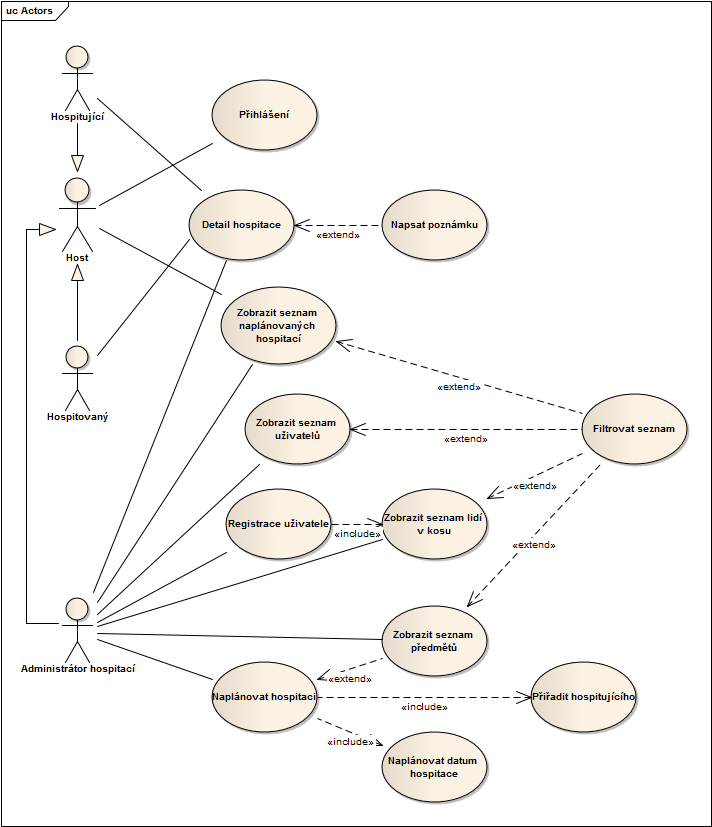
\includegraphics[width=10cm]{figures/Actors}
\caption{Aktéři}
\label{fig:actors}
\end{center}
\end{figure}

\subsection{Nepřihlášený uživatel}
Nepřihlášený uživatel je role pro hosty naší aplikace. V systému má ze všech rolí nejmenší pravomoc. V tomto stavu je každý uživatel, který se doposud nepřihlásil do systému.

\begin{figure}[H]
\begin{center}
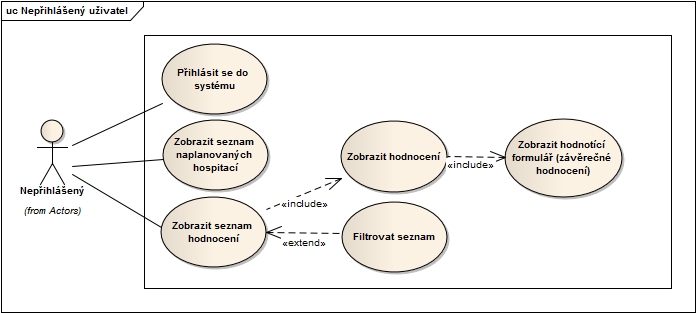
\includegraphics[width=10cm]{figures/actor_base}
\caption{Use case - nepřihlášený uživatel}
\label{fig:actor_base}
\end{center}
\end{figure}

\subsection{Přihlášený uživatel}
Přihlášený uživatel vychází z role nepřihlášeného uživatele. Je to uživatel, který se do systému přihlásil. Jedná se o základní roli pro všechny další role, které ji rozšiřují.

\begin{figure}[H]
\begin{center}
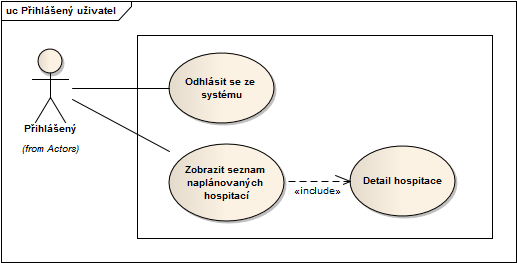
\includegraphics[width=10cm]{figures/actor_logged}
\caption{Use case - přihlášený uživatel}
\label{fig:actor_logged}
\end{center}
\end{figure}


\subsection{Hospitovaný}
Hospitovaný je role pro přihlášeného uživatele v systému. Je přidělena pro každého vyučujícího, který vyučuje předmět, na němž byla naplánovaná hospitace a proběhla.

\begin{figure}[H]
\begin{center}
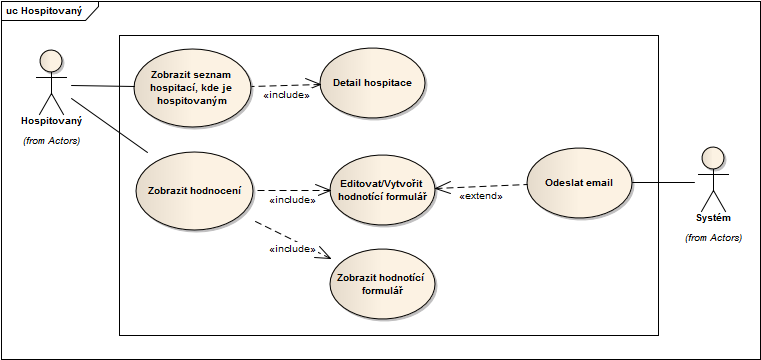
\includegraphics[width=10cm]{figures/actor_observed}
\caption{Use case - hospitovaný}
\label{fig:actor_observed}
\end{center}
\end{figure}

\subsection{Hospitující}
Hospitující je role pro přihlášeného uživatele v systému. Tato role se přiděluje automaticky z naplánovaných hospitací, nebo ji může přidělit administrátor hospitací.

\begin{figure}[H]
\begin{center}
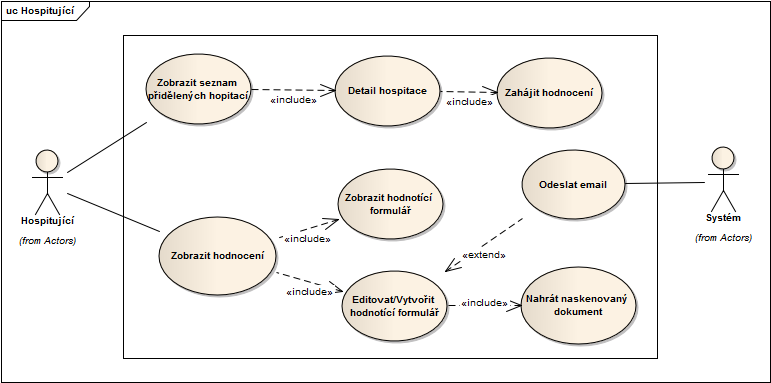
\includegraphics[width=10cm]{figures/actor_observer}
\caption{Use case - hospitující}
\label{fig:actor_observer}
\end{center}
\end{figure}

\subsection{Administrátor hospitací}
Hlavním úkolem této role je plánovat hospitace na předměty a posléze je spravovat.

\begin{figure}[H]
\begin{center}
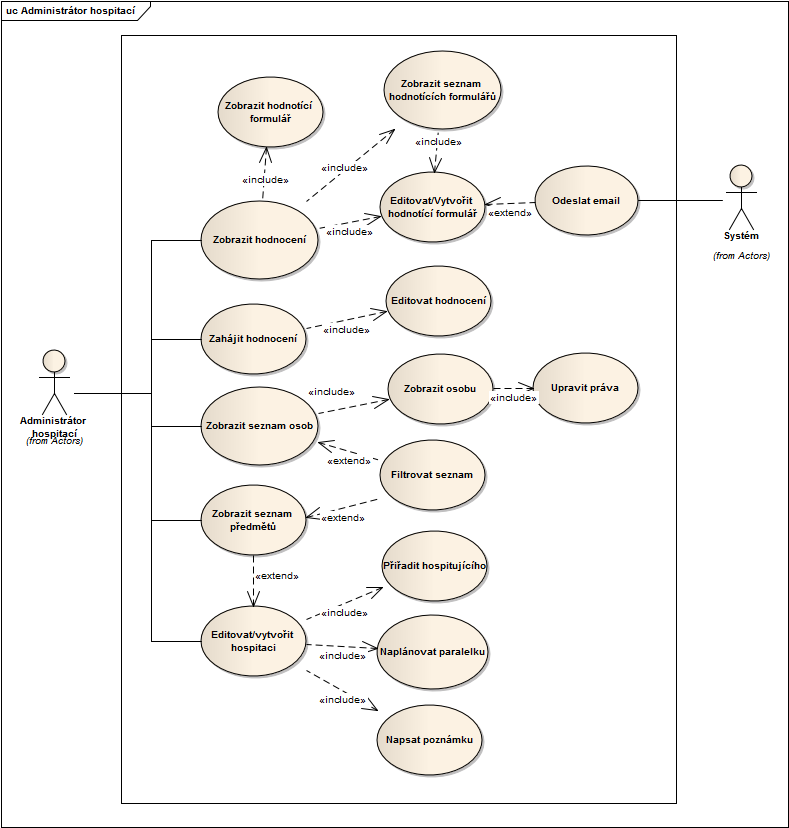
\includegraphics[width=10cm]{figures/actor_admin}
\caption{Use case - administrátor hospitací}
\label{fig:actor_admin}
\end{center}
\end{figure}

\subsection{Administrátor}
Administrátor je super uživatel, který má nejvyšší pravomoc v systému. Má přístup ke všem zdrojům aplikace a může aplikaci spravovat.

\begin{figure}[H]
\begin{center}
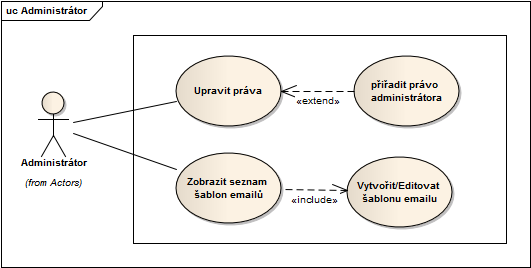
\includegraphics[width=10cm]{figures/actor_root}
\caption{Use case - administrátor}
\label{fig:actor_root}
\end{center}
\end{figure}

\newpage 
\section{Doménový model}
Doménový model na obrázku \ref{fig:domainmodel} reprezentuje entity v systému a jejich vzájemné vztahy. 

Popis domény jsem pro přehlednost rozdělil podle zdroje na dvě základní skupiny. V první skupině jsou domény, které jsem převzal ze struktury KOSapi a druhou skupinou jsou domény specifické pro moji aplikaci. 

\label{sec:domeny_kosapi} 
\subsection{Domény z KOSapi}
\begin{itemize}
\item Osoba - je osoba v KOSu. Každá osoba může být učitelem a studentem.
\item Semestr - semestr vyučovaný na FEL. 
\item Předmět - předměty vyučované na FEL.
\item Instance předmětu - jsou instance předmětu vypsané v konkrétním semestru.
\item Paralelka - je vypsaná rozvrhová paralelka pro instanci předmětu.
\item Místnost - místnost na FEL
\end{itemize}

\subsection{Domény aplikace}
\begin{itemize}
\item Hospitace - obsahuje informace o naplánování hospitace. 
\item Poznámka - je textová poznámka k plánování hospitace.
\item Hodnocení - reprezentuje informace z proběhlé hospitace hospitace, jsou to informace o datu vykonání hospitace, hospitujícím, předmětu a garantovi.
\item Příloha - je připojený datový soubor k hodnocení hospitace.
\item Šablona formuláře - šablona pro tvorbu formulářů. Definuje vlastnosti jakým se budou vytvářet hodnotící formuláře.
\item Položka - položka reprezentuje jednotlivé segmenty formuláře. Tyto segmenty pak v celku definují strukturu formuláře.
\item Formulář - vyplněný hodnotící formulář.
\item Hodnota - je hodnota z vyplněného formuláře. Ta se ukládá z položky formuláře.
\item Šablona emailu - šablona emailu ze které se budou generovat emailové zprávy.
\end{itemize}

\begin{figure}[p]
\begin{center}
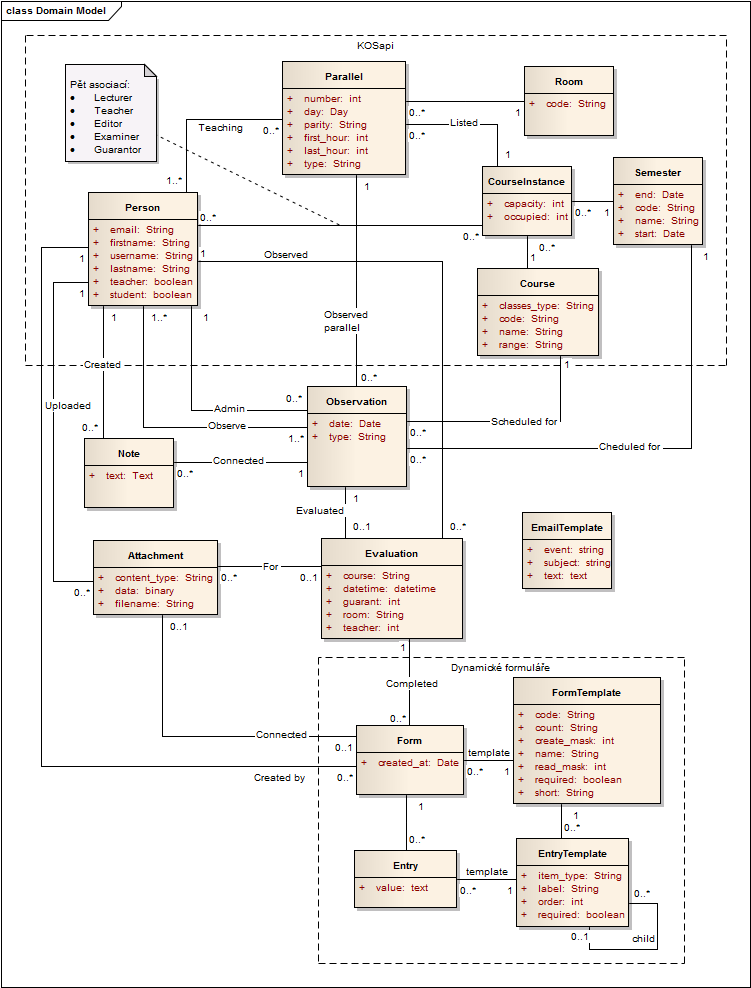
\includegraphics[width=14cm]{figures/DomainModel2}
\caption{Doménový model}
\label{fig:domainmodel}
\end{center}
\end{figure}



\section{Životní cyklus hospitace}
Cílem této části analýzy je popsat životní cyklus, kterým hospitace prochází. 

\subsection{Vytvoření}
Životní cyklus hospitace začíná jejím vytvořením. Toto zajišťuje administrátor hospitací, který založí hospitaci a definuje semestr, kdy se má hospitace uskutečnit, a předmět vyučovaný na fakultě. Při vytváření hospitace se určí typ hospitace a tím i její způsob zviditelnění, pro ostatní aktéry v aplikaci.

\subsection{Naplánování}
Při plánování je také hlavním aktérem administrátor hospitace. V této části životního cyklu administrátor určí hospitovanou paralelku předmětu a datum,  kdy se hospitace uskuteční.  

Administrátor také v této fázi přidělí hospitující z řad pedagogů určených k vykonání hospitace.  
 
\subsection{Hodnocení}
Poté, co proběhla kontrola hospitace, začíná nová fáze, ve které se hodnotí vyučování. Do této fáze už nezasahuje administrátor hospitace, ale přicházejí na scénu dva jiní aktéři: hospitovaný a hospitující.

V první fázi musí hospitující vyplnit, nebo nahrát naskenovaný formulář pro Hodnocení výuky při hospitaci. Tento formulář slouží k dokumentaci průběhu hospitace.

V druhé fázi jeden z hospitujících sepíše slovní hodnocení hospitační návštěvy.

Ve třetí fázi může hospitovaný do dvou dnů vyplnit stanovisko hodnoceného k názorům hospitujícího.  

V poslední fázi jeden z hospitujících sepíše poslední formulář Závěrečné shrnutí. Po vyplnění tohoto formuláře se hospitace stává ukončenou a tím končí její životní cyklu.
 
\subsection{Ukončená}
Po sepsáním posledního hodnotícího dokumentu se hospitace dostane do fáze ukončená. 

\begin{figure}[h]
\begin{center}
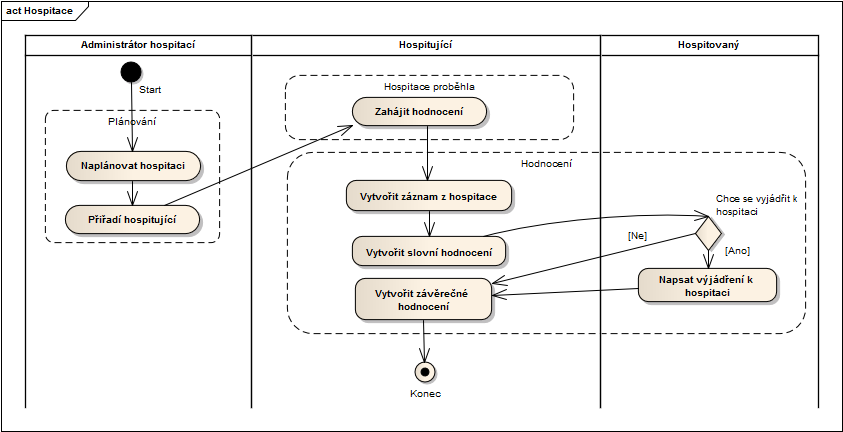
\includegraphics[width=14cm]{figures/hospitace}
\caption{Život hospitace}
\label{fig:hospitace}
\end{center}
\end{figure}


%*****************************************************************************
\chapter{Realizace}
Po dohodě s vedoucím práce byl zvolen iterační vývoj aplikace. Za účelem postupného vyvíjený částí aplikace, tak aby bylo možné testovat aplikaci na letním semestru 2011/2012. V této kapitole popisuji jednotlivá zadání každé iterace. Jak jsem postupoval k vyřešení zadání a výstupy z jednotlivých iterací. Jednotlivé iterace byly prezentovány na konzultacích s vedoucím práce.

\section{První iterace}
\subsection{Zadání}
Tato iterace patřila k nejobsáhlejším ze všech iterací. Jedním z důvodů bylo  seznámení se s novou technologii Ruby on Rails. První iterace měla za cíl navrhnout a vytvořit základní architekturu aplikace s napojením na KOSapi viz. \ref{kosapi} a k tomu vytvořit funkční část aplikace pro plánování hospitací, tak abych mohl prezentovat funkčnost.

\subsection{Postup}
\subsubsection{Datová vrstva}
Protože aplikace využívá dva datové zdroje KOSapi  a databázi aplikace, bylo potřeba nejdřív vyřešit jak se připojit ke KOSapi. V této části vycházím z prototypu aplikace pro správu hospitací. Ta využívá již naprogramovanou knihovnu z projektu VyVy \cite{vyvy}. Poté bylo potřeba vytvořil modely tak, aby umožnily komunikaci mezi KOSapi a databází aplikace. Při implementování knihovny do aplikace jsem musel vyřešit lokalizaci jazykových konstant v datech získaných z API. Řešení bylo jednoduché, stačilo rozšířit knihovnu o podporu knihovny i18n\footnote{lokalizace softwaru pro různé jazyky a jejich místních zvyklostí}, který je součástí Rails.

\subsubsection{Autentizace}
Pro autentizaci, v této fázi vývoje, používám knihovnu \textit{Authlogic}, kterou jsem zprovoznil pomocí návodu \cite{authlogic}. Tuto knihovnu používám jen dočasně po dobu vývoje aplikace. Ve finální fázi bude nahrazen autentizační službou FELid viz. \ref{felid}, kterou lze zprovoznit jen na serveru, kde bude aplikace nasazena. 

\subsubsection{Autorizace}
Autentizace v hospitacích je jedena z kritických oblastí, kterou bylo potřeba vyřešit hned na začátku vývoje. V aplikaci potřebuji autorizovat uživatele jak podle role, tak i podle vztahu k hospitaci. Proto jsem hledal modul, který by dokázal nadefinovat pravidla autorizace. Knihovna, kterou jsem použil, se jmenuje \textit{CanCan} \cite{cancan} . Tato knihovna má velmi jednoduchý, ale i přesto flexibilní zápis pravidel. Tyto pravidla umí filtrovat jak podle zdroje, tak i podle jednotlivých instancí záznamů. Umí také dokáže filtrovat metody v kontrolorech i celé zdroje aplikace. Veškerá pravidla jsou definována na jednom místě\footnote{model Ability} aplikace.

\begin{quote}
Příklad zapsaného pravidla pro administrátora hospitací pomocí knihovny \textit{CanCan} ve třídě modelu Ability. První pravidlo \verb|can| umožní zobrazovat, vytvářet, upravovat a mazat ze zdroje \textit{Observation}. Zároveň druhé pravidlo \verb|cannot| zakáže operace pro správu záznamů, které administrátor hospitací nevytvořil.

\begin{verbatim}
def admin
    can :manage, Observation
    cannot :manage, Observation do |ob|
        !(ob.created_by==current_user)
    end
end
\end{verbatim} 
\end{quote}

\subsubsection{Role}
\label{sec:role}
Role pro jednotlivé uživatelé uchovávám v modelu \textit{Role}. Kde jednotlivé role uživatele ukládám do jednoho atributu \verb|roles_mask| pomocí bitové masky. V bitové masce jsou reprezentovány role čísly mocniny 2. Díky tomu lze skládat role pomocí bitové operace OR. V tabulce \ref{tab:role} je přehled rolí s číslem reprezentující bitovou masku pro roli.

\begin{table}[h]
\begin{center}
\begin{tabular}{|l|c|}

\hline
\textbf{Role} & \textbf{Bitová maska} \\ \hline
Administrátor hospitací & 1 \\
Hospitující & 2 \\ 
Hospitovaný & 4 \\
Admin & 8 \\\hline

\end{tabular}
\caption{Reprezentace rolí v bitové masce}
\label{tab:role}
\end{center}
\end{table}

\subsubsection{Uživatelské prostředí}
Pro vytvoření uživatelského prostředí jsem použil již existující knihovnu \textit{Bootstrap} \cite{bootstrap}. Použil jsem tuto knihovnu abych si usnadnil implementaci uživatelského prostředí. Knihovna obsahuje kompletní CSS tak i JavaScriptové moduly. Mezi další výhody patří open-source licence a další výhodou je známé uživatelské prostředí používané ve webové aplikaci Twitter.

Pro usnadnění implementace knihovny \textit{Bootstrap} do aplikace jsem použil další dvě knihovny. První je modul \textit{SimpleForm} \cite{simpleform}, který slouží k vytváření formulářů. Základním cílem je nadefinovat rozvržení všech formulářů na jednom místě. Druhým modulem je \textit{WillPaginate} \cite{willpaginate} pro stránkování dat.

\subsection{Výstup} 
Výstupem z první iterace vznikla část aplikace, která uměla plánovat hospitace a uměla získávat data z webové služby KOSapi.


\section{Druhá iterace}
\subsection{Zadání}
Zadáním druhé iterace bylo na-implementovat hodnotící formuláře hospitací. Požadavkem byla možnost upravovat formuláře bez zásahu do zdrojového kódu aplikace. Dalším cílem bylo třeba vyřešit problém s KOSapi, který vznikl při přechodu na nový semestr. Služba neudržuje data instancí předmětů z minulých semestrů a proto nebylo možné získat všechny potřebné informace pro hospitace z minulých semestrů.

\subsection{Postup}
\subsubsection{Datová vrstva}
Problém se ztrátou dat byl velmi vážný, proto bylo potřeba tento problém rychle vyřešit, abych mohl pokračovat dále ve vývoji. Musel jsem proto předělat datovou část. Rozšířil jsem databázi o entity z kapitoly \ref{sec:domeny_kosapi} tak, aby data z KOSapi byla uložena v databázi. Data je potřeba synchronizovat v databázi s KOSapi. O synchronizaci se starájí \textit{rake}\footnote{rake je sada nástrojů používaná pro vývoj a nasazení Rails aplikací} scripty, které přidávají nové záznamy nebo je aktualizují. Synchronizační scripty se spouštějí každý den pomocí programu \textit{Cron}\footnote{Cron je program, který na pozadí operačního systému spouští naplánované úlohy}.

Po přidání nových entit bylo potřeba na-implementovat asociace mezi novými entitami. V modelu KOSapi je spousta asociací mezi entitami osoba - paralelka a osoba - instance předmětu. V aplikaci jich celkem používám šest. Všechny tyto asociace\footnote{asociace garant, přednášející, vyučující, instruktor a zkoušející.} mají kardinalitu N:M. Pokud bych použil klasickou dekompozicí přes pomocnou tabulku, která rozloží asociace na 1:N a 1:M. Vzniklo by mi šest pomocných tabulek. Proto jsem se rozhodl použít jiný způsob dekompozice přes polymorfní asociace \cite{guide_pa} v Ruby on Rails. Výhodou tohoto řešení je redukce počtu pomocných tabulek. Polymorfní asociace zredukoval počet ze šesti na jednu tabulku viz obrázek \ref{fig:polymorfni}. V tabulce \ref{tab:people_related} jsou popsány jednotlivé atributy pomocné tabulky \textit{PeopleRelated} s příklady hodnot.

\begin{figure}[h]
\begin{center}
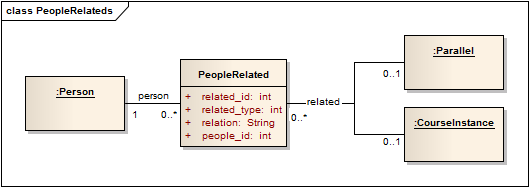
\includegraphics[width=12cm]{figures/PeopleRelateds}
\caption{Dekompozice pomocí polymorfní asociace}
\label{fig:polymorfni}
\end{center}
\end{figure}

\begin{table}[h]
\begin{center}
\begin{tabular}{|l|c|l|}

\hline
\textbf{Atribut} & \textbf{Příklad} & \textbf{Popis} \\ \hline
related\_id & 1 & cizí klíč záznamu, který je v asociaci s osobou \\\hline
related\_type & Parallel & jméno modelu ke kterému patří cizí klíč \\ & & v attributu \textit{related\_id} \\ \hline
relation & teachers & název asociace \\\hline
people\_id & 100 & cizí klíč pro osobu  \\\hline

\end{tabular}
\caption{Popis atributů tabulky PeopleRelated}
\label{tab:people_related}
\end{center}
\end{table}


\subsubsection{Hodnotící formuláře}
Z důvodu možné změny hodnotících formulářů v budoucnosti, jsem vytvořil návrh, který umožní vytvářet nové typy formulářů, nebo upravovat již existující. Formuláře se definují šablonou. Tato šablona definuje základní vlastnosti: minimální, maximální počet vyplnění, název a kdo může formulář vyplnit. Samotný obsah šablony formuláře se skládá z položek. Položky formuláře mohou být hodnotící tabulka, nadpis, hodnocení, text a jiné. Na obrázku \ref{fig:dynamicform} je doménový model dynamický formulářů. 

\begin{figure}[h]
\begin{center}
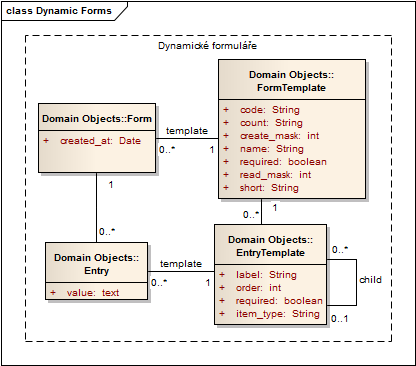
\includegraphics[scale=0.6]{figures/DynamicForms}
\caption{Doménový model dynamických formulářů}
\label{fig:dynamicform}
\end{center}
\end{figure}

Hodnotící formuláře se generují podle šablony formuláře získané z databáze. Šablona je reprezentovaná modelem \textit{FormTemplate}. Obsahuje veškeré informace potřebné pro formulaci chování formuláře. Mezi základní vlastnosti, které definuje šablona, patří název, popis a kód. Kód šablony je velmi důležitá vlastnost, definuje skupinu kam patří formulář. Skupiny formulářů jsou rozděleny podle druhu formuláře a ty popisuji v sekci hodnocení výuky \ref{sec:formulare}. Rozdělení formulářů do skupin s kombinací data vytvoření využívám pro verzování šablon. Šablony musím verzovat, jinak by mi při úpravě nebo smazání existující šablony, mohla nastat ztráta dat z  dříve vyplněných formulářů.

%Formuláře jsou rozděleny do skupin protože se časem mohou upravovat a nemůžu si dovolit upravit již vytvořenou šablonu. Mohlo by nastat ztráta dat ve vyplněných formulářích, proto se musí vždy vytvořit nová šablona.  

Šablona formuláře definuje také postupné hodnocení. Pro otevření dalšího typu formuláře se musí splnit několik podmínek:

\begin{enumerate}
\item Povinný formulář musí být vyplněn a také musí splnit podmínku pro minimální počet. V jiném případě není potřeba vyplnit žádný jiný formulář.
\item Minimální počet lze definovat buď přesným počtem, nebo dynamicky podle asociace. Kde minimální počet mi definuje počet instancí v asociaci. Počet vytvořených formulářů se počítá pouze z jednoho hodnocení hospitace.
\item Hospitující i hospitovaný může vyplnit maximálně jeden formulář.
\end{enumerate}

U dynamických formulářů jsem musel také řešit jejich chování pro různé role v systému. Proto jsem přidal do šablony dva atributy s bitovými maskami rolí jedna maska pro role, které mohou zobrazit formulář, druhá maska pro vyplnění formuláře. Používám stejný způsob rozlišování rolí v bitové masce jako u rolí pro uživatele viz \ref{sec:role}.

Obsah formuláře generuji pomocí položek, ty jsou reprezentovány modelem \textit{EntryTemplate}. Položky formuláře definují co se má vykreslit a kde. Umístění jednotlivých položek v dokumentu je definované ve stromové struktuře, kde kořenem stromu je šablona formuláře a ta se postupně větví přes instance modelu \textit{EntryTemplate}. Co se má vykreslit je definované atributem typ elementu. Na obrázku \ref{fig:tree_form} je zobrazen příklad stromové struktury s typy elementů. Příloha \ref{sec:forms} dokumentu obsahuje  seznam všech podporovaných typů elementů a jejich vlastnosti v tabulce i s obrázkem se sestaveným formulářem s rozložením typů elementů. Samotné generování obsahu není složitý proces. Celý formulář se sestaví hierarchicky i s hodnotami z modelu \textit{Entry}.

\begin{figure}[h]
\Tree [.FormTemplate [.EntryTemplate\\(ranking\_table) [.EntryTemplate\\(ranking) ][.EntryTemplate\\(ranking) ]] [.EntryTemplate\\(text) ] [.EntryTemplate\\(label) ]]

\caption{Příklad stromové struktury formuláře}
\label{fig:tree_form}
\end{figure}

Nestačí nám pouze vygenerovat formulář, ale potřebujeme i uložit jeho hodnoty do databáze. O to se starají modely \textit{Form} a \textit{Entry}. Model \textit{Form} složí pro identifikaci konkrétního vyplněného formuláře. Jednotlivé hodnoty z vyplněného formuláře jsou uložené v \textit{Entry} viz obrázek \ref{fig:data_form}.

\begin{figure}[h]
\Tree [.Form [.Entry\\(A) ] [.Entry\\(B) ] [.Entry\\(text) ]]
\caption{Příklad uložených dat}
\label{fig:data_form}
\end{figure}
%[.Entry [.B]] [.Entry [.text]]
\subsection{Výstup} 
Výstupem této iterace byla aplikace, která již využívala pouze svoji databázi pro zdroj dat z KOSu a dynamické formuláře s nadefinovanými šablonami formulářů. 

\section{Třetí iterace}
\subsection{Zadání}
Zadáním třetí iterace bylo připravit server pro službu FELid. Dalším požadavkem bylo zprovoznění automatického zálohování databáze.

\subsection{Postup}
\subsubsection{Nasazení aplikace}
Na diagramu nasazení \ref{fig:deployment} jsou znázorněny komponenty potřebné pro nasazení aplikace. Protože na serveru byl nainstalován pouze webový server Apache HTTP Server a databázový systém Mysql, bylo potřeba nainstalovat platformu Ruby a framework Ruby on Rail. K instalaci Ruby jsem se rozhodl použít software RVM. Instalaci jsem provedl podle návodu pro více uživatelskou instalaci \cite{RVM}. Tento program dovolí nainstalovat různé platformy Ruby na jednom počítači. Další přínosem je spravování gemsets\footnote{balíky knihoven mezi kterými lze přepínat pro různé aplikace}, díky nimž lze zprovoznit několik aplikací zároveň na jednom počítači. Do nainstalovaného webového serveru bylo potřeba ještě přidat zásuvný modul, který umožní nasadit Rails aplikace. Modul se jmenuje Passanger (mod\_rails) a instaloval jsem ho do Apache podle návodu na oficiálních stránkách \cite{passenger}.

\subsubsection{FELid}
Pro zprovoznění služby FELid, bylo potřeba splnit několik požadavků. Tyto požadavky jsou umístěny na oficiálních stránkách služby \cite{felid_pozadavky}. Jeden z požadavků je zprovoznění programu, který zajistí komunikaci se službou FELid. Tento program se jmenuje Shibboleth a obsahuje zásuvný modul mod\_shib do webového serveru. Při konfiguraci programu jsem postupoval podle návodu, který se nachází na wiki stránkách FELid \citep{felid}. Po splnění všech požadavků stačilo jen zažádat o registraci aplikace.

\begin{figure}[h]
\begin{center}
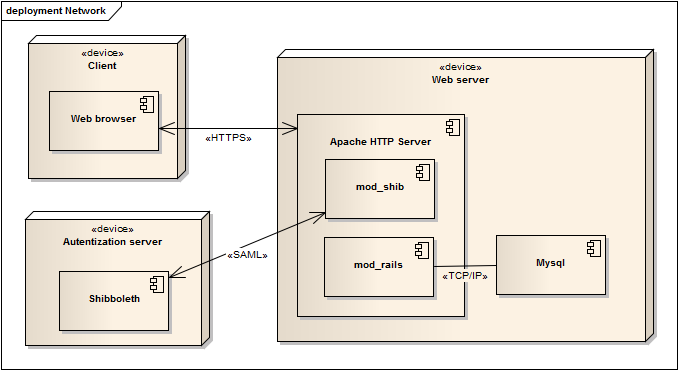
\includegraphics[width=12cm]{figures/deployment}
\caption{Diagram nasazení}
\label{fig:deployment}
\end{center}
\end{figure}

\subsubsection{Zálohavání databáze}
Pro automatické zálohování databáze jsem použil existující řešení  Ruby aplikace \textit{Backup} pro zálohování databází. Tato aplikace každý den vytvoří zálohu databáze, kterou uloží na disk. Na disku uchovává 300 záloh databáze, při překročení počtu záloh se starší zálohy nahrazují novými. Výhodou tohoto řešení je podpora různých databázových systémů a možnost ukládat zálohy na externí uložiště\footnote{pro příklad Amazon Simple Storage Service (S3)}. Záloha se spouští pravidelně pomocí programu \textit{Cron} každý den brzy ráno příkazem:
\begin{verbatim}
backup perform --trigger backup
\end{verbatim} 

\subsection{Výstup} 
V této iteraci se mi podařilo zprovoznit aplikaci na serveru a otestovat její funkčnost. Také jsem pracoval na programu, který jsem upravoval podle získaných připomínek od zadavatele z minulých iterací.

\section{Čtvrtá iterace}
\subsection{Zadání}
Tato iterace je poslední a proto většinu zadání tvořily připomínky od zadavatele. V této iteraci patří mezi hlavní úkoly vytvoření modulu, který bude generovat emailové zprávy po vyplnění hodnotícího formuláře a integrovat autentizaci přes FELid. 
\subsection{Postup}
\subsubsection{Autentizace}
V této fázi vývoje byla aplikace zaregistrována ve FELid. Před integrováním autentizace přes FELid, je potřeba otestovat aplikaci. Nejdůležitější je otestovat správnou funkčnost autorizace u všech rolí v celém systému. Po zprovoznění autentizace přes FELid není možné jednoduše testovat aplikaci pod různými uživateli. Od zprovoznění nebudu mít totiž kontrolu nad autentizací.

Integrace do aplikace je pak velmi jednoduchá. Stačilo jen odstranit dočasný způsob autentizace, který jsem implementoval v první iteraci. Aplikace FElid poskytuje aplikaci informace o přihlášeném uživateli prostřednictvím atributů v proměnné \verb|request.env|. Pro identifikaci přihlášeného uživatele používám atribut \verb|felid-uid| ve kterém se nachází uživatelské jméno. Autentizaci v aplikaci se stará jen jedna funkce \verb|current_user_session|.

\begin{quote}
\begin{verbatim}
def current_user_session
    return @user if defined?(@user)
    if not request.local? and not request.env["felid-uid"].nil? 
      and @user.nil? 
    then
      @user = People.find_by_username request.env["felid-uid"]
    end
    return @user
end
\end{verbatim} 
\end{quote}

\subsubsection{Emaily}
Jeden z požadavků bylo odesílání emailových zpráv po vyplnění hodnotícího formuláře. Součástí zadání je generování emailů ze šablon. Šablona se skládá z předmětu, textu zprávy a názvu akce. Akce v systému mohou být různých druhů, podle zadání stačilo pouze implementovat akce pro vytvoření formulářů. Při vykonání akce se vygeneruje emailová správa ze šablony emailu.

\subsubsection{Generátor obsahu emailových zpráv}
Protože je potřeba generovat do emailu proměnná data z hospitací, tak jsem vytvořil knihovnu \textit{EmailTemplates} pro generování obsahu emailů. Úkolem modulu je nahradit značky v textu za skutečná data. Pro vložení generovaných dat se používá zápis \verb|%značka%| do textu zprávy. 
\begin{quote}
Příklad vygenerování jednoduchého emailu se značkou pro kód předmětu.
\begin{verbatim}
text %course_code% => text A7B36ASS
\end{verbatim} 
\end{quote}

Při vývoji modulu jsem si dal za cíl vytvořit takovou knihovnu, která by umožnila jednoduše nastavit podporované značky. Největším zádrhelem v generování obsahu zprávy je získat data z hospitací. Protože vstupem do generátoru používám pouze instanci šablony a hodnocení hospitace, tak některá data musím získat přes několik relací mezi modely.

Knihovna obsahuje dva moduly. První částí je modul \textit{ModelHelper}, který slouží pro rozšíření libovolné třídy modelu v aplikaci. Rozšířenému modelu umožní pomocí statické metody \verb|attrs_tagged(*args)| povolit atributy ze kterých bude generátor získávat data. 

\begin{quote}
Příklad jednoduchého nastavení modelu \textit{Person}, které umožní generátoru vkládat jméno, emailovou adresu a uživatelské jméno.
\begin{verbatim}
class Person < ActiveRecord::Base
  include EmailTemplates::Tagged::ModelHelpers
    attrs_tagged :name, :email, :username
end
\end{verbatim} 
\end{quote}

Druhou částí je modul \textit{EmailBuilder}. Tento modul slouží pro vytvoření vlastního generátoru pomocí jednoduchého nastavování. Pro tyto účely modul poskytuje statickou metodu \verb|source(model,name,*path)|, ta slouží pro nastavení zdroje dat. Metoda dynamicky rozšíří třídu o metodu, ta dokáže získat data z aplikace. Využívá k tomu nastavení z modelu rozšířeného pomocí \textit{ModelHelper} a cesty k instancím modelu s daty. Cesta je definována posloupností názvů asociací mezi modely. 

\begin{quote}
Příklad implementace jednoduchého generátoru \textit{EmailBuilder}, který dokáže vkládat do emailů informace o hospitovaném učiteli. 
\begin{verbatim}
class EmailBuilder
  include Tagged::EmailBuilder
  source Person, :teacher, :evaluation, :teacher
end
\end{verbatim} 
Tento generátor bude podporovat tři značky \verb|%teacher_name%|, \verb|%teacher_email%| a \verb|%teacher_username%|. Tímto způsobem lze jednoduše nadefinovat velké množství značek.
\end{quote}

Struktura značky \ref{fig:znacka} se skládá ze dvou základních částí, ze jména zdroje a jména atributu, ze kterého generátor získá data pro nahrazení značky. 
\begin{figure}[h]
\Tree [.\%teacher\_name\% [.teacher (zdroj) ]  [.name (atribut) ] ]
\caption{Struktura značky}
\label{fig:znacka}
\end{figure}

Výhodou této knihovny je krátký a jednoduchý zápis pro vytvoření vlastního generátoru, který dokáže přes asociace mezi modely získávat data. V aplikaci jsem celkem nadefinoval pro devět zdrojů 32 značek.
 
\subsubsection{Odesílání emailů}
Dle zadání stačilo implementovat odesílání zpráv po vytvoření hodnotícího formuláře. Podle druhu hodnotícího formuláře se vygeneruje zpráva a odešle se administrátorovi hospitace, hospitujícím, hospitovaným garantovi předmětu a vedoucímu katedry. Do budoucna lze rozšířit v aplikaci odesílání emailů i při jiných akcí. Pro příklad se mohou odesílat při naplánování nové hospitace. 

Z časových a technických problémů se mi nepodařilo zprovoznit emailový server pro odesílání emailů, proto dočasně používám k odesílání emailový účet kvalitavyuky.gmail.com na Gmail.

\subsection{Výstup}
Výstupem z této iterace je finální aplikace, která splňuje všechny hlavní požadavky na funkčnost. 

%*****************************************************************************
\chapter{Testování}

Cílem testování bylo otestovat reálnou funkčnost aplikace a odhalit vzniklé chyby  při vývoji aplikace. Aplikaci jsem testoval dvěma způsoby manuálně, kde jsem musel ručně procházet aplikaci a zkoušet její funkčnost, a  Funkčnost aplikace jsem testoval manuálně a automaticky pomocí testovacích nástrojů v Ruby on Rails. Aplikaci jsem testoval v průběhu celého vývoje.  

\section{Automatické testování}
Automatické testy je důležité používat na místech, kde je velké riziko vzniku chyb. Nejčastější vznikají chyby při přidávání, nebo úpravě funkcionality.
Pro automatické testování jsem použil testovací nástroje v Ruby on Rails.
V Ruby on Rails se testy dělí do tří kategorií.

\subsection{Testovací data}
Pro automatické testování je potřeba připravit testovací data. Testovací data jsou obsažená ve struktuře programu pod tests/fixtures. Zde se pak nacházejí Soubory s testovacími daty pro jednotlivé modely ve formátu YAML.

\subsection{Unit testing}
Unit testy slouží k testování samostatných částí programů. V Rails se Unit testy používají hlavně pro testování funkčnosti modelů. Testuje se hlavně validace vstupů a perzistence dat.

\subsection{Functional tests}
Tyto testy testůjí rozné činnosti v jednotlivých controllerech aplikace. Controllery zpracovávají příchozí webové requesty a nakonec odpoví vyrendrovaným pohledem. Tento typ testů testuje:

\begin{list}{•}{}
\item Byl webový požadavek úspěšný?
\item Byli jsme přesměrováni na správnou stránku?
\item Byli jsme úspěšně přihlášeni?
\item Byl objekt vložen do správné šablony?
\item Byla zobrazena správná hláška uživateli?
\end{list} 

\subsection{Integration testing}
Integrační testy se používají k testování interakce mezi libovolným počtem kontrolorů. Obvykle se používají k testování důležitých pracovních toků v rámci aplikace.

\section{Manuální testování}
Manuálně jsem testoval části aplikace u kterých se špatně vytvářejí automatické testy, nebo byl potřeba lidský úsudek\footnote{testování uživatelského prostředí}. Primárně jsem testoval reálnou funkčnost aplikace na konci každé iterace. Procházel jsem aplikaci podle scénářů užití a využíval jsem reálná data z probíhajících hospitací v letním semestru 2011/2012.


%*****************************************************************************
\chapter{Závěr}

Výstupem mé práce je aplikace pro evidenci hospitací. Aplikace je nasazená na serveru
http://kvalitavyuky.felk.cvut.cz tak, že ji lze použít v reálném provozu na ČVUT FEL. Samotná aplikace byla implementovaná na platformě Ruby on Rails, což je jeden z nejmodernějších frameworků pro vývoj webových aplikací. Aplikace používá dvě fakultní aplikace. Pro autentizaci používá aplikaci FELid, což je globální autentizační systém pro webové aplikace na fakultě FEl. Druhou aplikací je KOSapi, ta poskytuje aplikační rozhraní k přístupu dat v KOSu.

Pro vývoj aplikace byl použit iterační vývoj, kdy při každé iteraci byly zpracovány požadavky zadavatele a následně byli zdokumentovány. Snažil jsem se vytvořit funkční a uživatelsky přívětivou aplikaci. Funkčnost aplikace jsem demonstroval simulací probíhajících hospitací pro studijní program STM v LS 2011/2012. Bohužel se nepodařilo v čas aplikaci nasadit do reálného provozu.

Tato práce mi přinesla spoustu zkušenosti jak s novou technologií Ruby on Rail, kterou jsem do té doby nepoužil, tak i s použitím externích aplikací.

\section{Možnosti v pokračování práce}
Možností pokračování v práci je několik. V první řadě je potřeba nainstalovat a nastavit na serveru emailový server pro odesílání informačních emailových zpráv.

Lze také pokračovat ve vývoji dynamických formulářů. Do aplikace jsem totiž neimplementoval uživatelské prostředí pro nastavování formulářů. Dále by bylo dobré předělat funkční část do knihovny. Jako dalším krokem pro vylepšení aplikace bych provedl refaktoring celé aplikace, protože při vývoji jsem se postupně učil pracovat v Ruby on Rails.


%*****************************************************************************
% Seznam literatury je v samostatnem souboru reference.bib. Ten
% upravte dle vlastnich potreb, potom zpracujte (a do textu
% zapracujte) pomoci prikazu bibtex a nasledne pdflatex (nebo
% latex). Druhy z nich alespon 2x, aby se poresily odkazy.

% originally following specification for bibliography formating was used
%\bibliographystyle{abbrv}

% Here is an improvment by Petr Dlouhy (April 2010).
% It is mainly for supervisors who expect Czech fomrating rules for references
% Additional feature is live url addresses to sources from your pdf file
% It requires the file csplainnat.bst (included in this sample zipfile).

\bibliographystyle{csplainnat}

%bibliographystyle{plain}
%\bibliographystyle{psc}
{
%JZ: 11.12.2008 Kdo chce mit v techto ukazkovych odkazech take odkaz na CSTeX:
\def\CS{$\cal C\kern-0.1667em\lower.5ex\hbox{$\cal S$}\kern-0.075em $}
\bibliography{reference}
}

% M. Dušek radi:
%\bibliographystyle{alpha}
% kdy citace ma tvar [AutorRok] (napriklad [Cook97]). Sice to asi neni  podle ceske normy (BTW BibTeX stejne neodpovida ceske norme), ale je to nejprehlednejsi.
% 3.5.2009 JZ polemizuje: BibTeX neobvinujte, napiste a poskytnete nam styl (.bst) splnujici citacni normu CSN/ISO.

%*****************************************************************************
%*****************************************************************************
\appendix

\chapter{Testování zaplnění stránky a odsazení odstavců}
\textbf{\large Tato příloha nebude součástí vaší práce. 
Slouží pouze jako příklad formátování textu.}

\section*{}
Určitě existuje nějaká pěkná latinská věta, která se k tomuhle testování používá, ale co mají dělat ti, kteří se nikdy latinsky neučili? Určitě existuje nějaká pěkná latinská věta, která se k tomuhle testování používá, ale co mají dělat ti, kteří se nikdy latinsky neučili? Určitě existuje nějaká pěkná latinská věta, která se k tomuhle testování používá, ale co mají dělat ti, kteří se nikdy latinsky neučili?

\begin{figure}[h]
\begin{center}

\includegraphics[width=14cm]{figures/LogoCVUT}
\caption{Aktéři}
\label{fig:actors}
\end{center}
\end{figure}


Určitě existuje nějaká pěkná latinská věta, která se k tomuhle testování používá, ale co mají dělat ti, kteří se nikdy latinsky neučili? Určitě existuje nějaká pěkná latinská věta, která se k tomuhle testování používá, ale co mají dělat ti, kteří se nikdy latinsky neučili? Určitě existuje nějaká pěkná latinská věta, která se k tomuhle testování používá, ale co mají dělat ti, kteří se nikdy latinsky neučili?

Určitě existuje nějaká pěkná latinská věta, která se k tomuhle testování používá, ale co mají dělat ti, kteří se nikdy latinsky neučili? Určitě existuje nějaká pěkná latinská věta, která se k tomuhle testování používá, ale co mají dělat ti, kteří se nikdy latinsky neučili? Určitě existuje nějaká pěkná latinská věta, která se k tomuhle testování používá, ale co mají dělat ti, kteří se nikdy latinsky neučili?

Určitě existuje nějaká pěkná latinská věta, která se k tomuhle testování používá, ale co mají dělat ti, kteří se nikdy latinsky neučili? Určitě existuje nějaká pěkná latinská věta, která se k tomuhle testování používá, ale co mají dělat ti, kteří se nikdy latinsky neučili? Určitě existuje nějaká pěkná latinská věta, která se k tomuhle testování používá, ale co mají dělat ti, kteří se nikdy latinsky neučili? Určitě existuje nějaká pěkná latinská věta, která se k tomuhle testování používá, ale co mají dělat ti, kteří se nikdy latinsky neučili? Určitě existuje nějaká pěkná latinská věta, která se k tomuhle testování používá, ale co mají dělat ti, kteří se nikdy latinsky neučili? Určitě existuje nějaká pěkná latinská věta, která se k tomuhle testování používá, ale co mají dělat ti, kteří se nikdy latinsky neučili?

Určitě existuje nějaká pěkná latinská věta, která se k tomuhle testování používá, ale co mají dělat ti, kteří se nikdy latinsky neučili? Určitě existuje nějaká pěkná latinská věta, která se k tomuhle testování používá, ale co mají dělat ti, kteří se nikdy latinsky neučili?

Určitě existuje nějaká pěkná latinská věta, která se k tomuhle testování používá, ale co mají dělat ti, kteří se nikdy latinsky neučili? Určitě existuje nějaká pěkná latinská věta, která se k tomuhle testování používá, ale co mají dělat ti, kteří se nikdy latinsky neučili? Určitě existuje nějaká pěkná latinská věta, která se k tomuhle testování používá, ale co mají dělat ti, kteří se nikdy latinsky neučili? Určitě existuje nějaká pěkná latinská věta, která se k tomuhle testování používá, ale co mají dělat ti, kteří se nikdy latinsky neučili? Určitě existuje nějaká pěkná latinská věta, která se k tomuhle testování používá, ale co mají dělat ti, kteří se nikdy latinsky neučili?

Určitě existuje nějaká pěkná latinská věta, která se k tomuhle testování používá, ale co mají dělat ti, kteří se nikdy latinsky neučili? Určitě existuje nějaká pěkná latinská věta, která se k tomuhle testování používá, ale co mají dělat ti, kteří se nikdy latinsky neučili? Určitě existuje nějaká pěkná latinská věta, která se k tomuhle testování používá, ale co mají dělat ti, kteří se nikdy latinsky neučili? Určitě existuje nějaká pěkná latinská věta, která se k tomuhle testování používá, ale co mají dělat ti, kteří se nikdy latinsky neučili? Určitě existuje nějaká pěkná latinská věta, která se k tomuhle testování používá, ale co mají dělat ti, kteří se nikdy latinsky neučili?

Určitě existuje nějaká pěkná latinská věta, která se k tomuhle testování používá, ale co mají dělat ti, kteří se nikdy latinsky neučili? Určitě existuje nějaká pěkná latinská věta, která se k tomuhle testování používá, ale co mají dělat ti, kteří se nikdy latinsky neučili? Určitě existuje nějaká pěkná latinská věta, která se k tomuhle testování používá, ale co mají dělat ti, kteří se nikdy latinsky neučili? Určitě existuje nějaká pěkná latinská věta, která se k tomuhle testování používá, ale co mají dělat ti, kteří se nikdy latinsky neučili? Určitě existuje nějaká pěkná latinská věta, která se k tomuhle testování používá, ale co mají dělat ti, kteří se nikdy latinsky neučili?

Určitě existuje nějaká pěkná latinská věta, která se k tomuhle testování používá, ale co mají dělat ti, kteří se nikdy latinsky neučili? Určitě existuje nějaká pěkná latinská věta, která se k tomuhle testování používá, ale co mají dělat ti, kteří se nikdy latinsky neučili? Určitě existuje nějaká pěkná latinská věta, která se k tomuhle testování používá, ale co mají dělat ti, kteří se nikdy latinsky neučili? Určitě existuje nějaká pěkná latinská věta, která se k tomuhle testování používá, ale co mají dělat ti, kteří se nikdy latinsky neučili? Určitě existuje nějaká pěkná latinská věta, která se k tomuhle testování používá, ale co mají dělat ti, kteří se nikdy latinsky neučili?

Určitě existuje nějaká pěkná latinská věta, která se k tomuhle testování používá, ale co mají dělat ti, kteří se nikdy latinsky neučili? Určitě existuje nějaká pěkná latinská věta, která se k tomuhle testování používá, ale co mají dělat ti, kteří se nikdy latinsky neučili? Určitě existuje nějaká pěkná latinská věta, která se k tomuhle testování používá, ale co mají dělat ti, kteří se nikdy latinsky neučili? Určitě existuje nějaká pěkná latinská věta, která se k tomuhle testování používá, ale co mají dělat ti, kteří se nikdy latinsky neučili? Určitě existuje nějaká pěkná latinská věta, která se k tomuhle testování používá, ale co mají dělat ti, kteří se nikdy latinsky neučili?

Určitě existuje nějaká pěkná latinská věta, která se k tomuhle testování používá, ale co mají dělat ti, kteří se nikdy latinsky neučili? Určitě existuje nějaká pěkná latinská věta, která se k tomuhle testování používá, ale co mají dělat ti, kteří se nikdy latinsky neučili? Určitě existuje nějaká pěkná latinská věta, která se k tomuhle testování používá, ale co mají dělat ti, kteří se nikdy latinsky neučili? Určitě existuje nějaká pěkná latinská věta, která se k tomuhle testování používá, ale co mají dělat ti, kteří se nikdy latinsky neučili? Určitě existuje nějaká pěkná latinská věta, která se k tomuhle testování používá, ale co mají dělat ti, kteří se nikdy latinsky neučili?

Určitě existuje nějaká pěkná latinská věta, která se k tomuhle testování používá, ale co mají dělat ti, kteří se nikdy latinsky neučili? Určitě existuje nějaká pěkná latinská věta, která se k tomuhle testování používá, ale co mají dělat ti, kteří se nikdy latinsky neučili? Určitě existuje nějaká pěkná latinská věta, která se k tomuhle testování používá, ale co mají dělat ti, kteří se nikdy latinsky neučili? Určitě existuje nějaká pěkná latinská věta, která se k tomuhle testování používá, ale co mají dělat ti, kteří se nikdy latinsky neučili? Určitě existuje nějaká pěkná latinská věta, která se k tomuhle testování používá, ale co mají dělat ti, kteří se nikdy latinsky neučili?

Určitě existuje nějaká pěkná latinská věta, která se k tomuhle testování používá, ale co mají dělat ti, kteří se nikdy latinsky neučili? Určitě existuje nějaká pěkná latinská věta, která se k tomuhle testování používá, ale co mají dělat ti, kteří se nikdy latinsky neučili? Určitě existuje nějaká pěkná latinská věta, která se k tomuhle testování používá, ale co mají dělat ti, kteří se nikdy latinsky neučili? Určitě existuje nějaká pěkná latinská věta, která se k tomuhle testování používá, ale co mají dělat ti, kteří se nikdy latinsky neučili? Určitě existuje nějaká pěkná latinská věta, která se k tomuhle testování používá, ale co mají dělat ti, kteří se nikdy latinsky neučili?

Určitě existuje nějaká pěkná latinská věta, která se k tomuhle testování používá, ale co mají dělat ti, kteří se nikdy latinsky neučili? Určitě existuje nějaká pěkná latinská věta, která se k tomuhle testování používá, ale co mají dělat ti, kteří se nikdy latinsky neučili? Určitě existuje nějaká pěkná latinská věta, která se k tomuhle testování používá, ale co mají dělat ti, kteří se nikdy latinsky neučili? Určitě existuje nějaká pěkná latinská věta, která se k tomuhle testování používá, ale co mají dělat ti, kteří se nikdy latinsky neučili? Určitě existuje nějaká pěkná latinská věta, která se k tomuhle testování používá, ale co mají dělat ti, kteří se nikdy latinsky neučili?

Určitě existuje nějaká pěkná latinská věta, která se k tomuhle testování používá, ale co mají dělat ti, kteří se nikdy latinsky neučili? Určitě existuje nějaká pěkná latinská věta, která se k tomuhle testování používá, ale co mají dělat ti, kteří se nikdy latinsky neučili? Určitě existuje nějaká pěkná latinská věta, která se k tomuhle testování používá, ale co mají dělat ti, kteří se nikdy latinsky neučili? Určitě existuje nějaká pěkná latinská věta, která se k tomuhle testování používá, ale co mají dělat ti, kteří se nikdy latinsky neučili? Určitě existuje nějaká pěkná latinská věta, která se k tomuhle testování používá, ale co mají dělat ti, kteří se nikdy latinsky neučili?

Určitě existuje nějaká pěkná latinská věta, která se k tomuhle testování používá, ale co mají dělat ti, kteří se nikdy latinsky neučili? Určitě existuje nějaká pěkná latinská věta, která se k tomuhle testování používá, ale co mají dělat ti, kteří se nikdy latinsky neučili? Určitě existuje nějaká pěkná latinská věta, která se k tomuhle testování používá, ale co mají dělat ti, kteří se nikdy latinsky neučili? Určitě existuje nějaká pěkná latinská věta, která se k tomuhle testování používá, ale co mají dělat ti, kteří se nikdy latinsky neučili? Určitě existuje nějaká pěkná latinská věta, která se k tomuhle testování používá, ale co mají dělat ti, kteří se nikdy latinsky neučili?

Určitě existuje nějaká pěkná latinská věta, která se k tomuhle testování používá, ale co mají dělat ti, kteří se nikdy latinsky neučili? Určitě existuje nějaká pěkná latinská věta, která se k tomuhle testování používá, ale co mají dělat ti, kteří se nikdy latinsky neučili? Určitě existuje nějaká pěkná latinská věta, která se k tomuhle testování používá, ale co mají dělat ti, kteří se nikdy latinsky neučili? Určitě existuje nějaká pěkná latinská věta, která se k tomuhle testování používá, ale co mají dělat ti, kteří se nikdy latinsky neučili? Určitě existuje nějaká pěkná latinská věta, která se k tomuhle testování používá, ale co mají dělat ti, kteří se nikdy latinsky neučili?

Určitě existuje nějaká pěkná latinská věta, která se k tomuhle testování používá, ale co mají dělat ti, kteří se nikdy latinsky neučili? Určitě existuje nějaká pěkná latinská věta, která se k tomuhle testování používá, ale co mají dělat ti, kteří se nikdy latinsky neučili? Určitě existuje nějaká pěkná latinská věta, která se k tomuhle testování používá, ale co mají dělat ti, kteří se nikdy latinsky neučili? Určitě existuje nějaká pěkná latinská věta, která se k tomuhle testování používá, ale co mají dělat ti, kteří se nikdy latinsky neučili? Určitě existuje nějaká pěkná latinská věta, která se k tomuhle testování používá, ale co mají dělat ti, kteří se nikdy latinsky neučili?

Určitě existuje nějaká pěkná latinská věta, která se k tomuhle testování používá, ale co mají dělat ti, kteří se nikdy latinsky neučili? Určitě existuje nějaká pěkná latinská věta, která se k tomuhle testování používá, ale co mají dělat ti, kteří se nikdy latinsky neučili? Určitě existuje nějaká pěkná latinská věta, která se k tomuhle testování používá, ale co mají dělat ti, kteří se nikdy latinsky neučili? Určitě existuje nějaká pěkná latinská věta, která se k tomuhle testování používá, ale co mají dělat ti, kteří se nikdy latinsky neučili? Určitě existuje nějaká pěkná latinská věta, která se k tomuhle testování používá, ale co mají dělat ti, kteří se nikdy latinsky neučili?

Určitě existuje nějaká pěkná latinská věta, která se k tomuhle testování používá, ale co mají dělat ti, kteří se nikdy latinsky neučili? Určitě existuje nějaká pěkná latinská věta, která se k tomuhle testování používá, ale co mají dělat ti, kteří se nikdy latinsky neučili? Určitě existuje nějaká pěkná latinská věta, která se k tomuhle testování používá, ale co mají dělat ti, kteří se nikdy latinsky neučili? Určitě existuje nějaká pěkná latinská věta, která se k tomuhle testování používá, ale co mají dělat ti, kteří se nikdy latinsky neučili? Určitě existuje nějaká pěkná latinská věta, která se k tomuhle testování používá, ale co mají dělat ti, kteří se nikdy latinsky neučili?

%*****************************************************************************
\chapter{Pokyny a návody k formátování textu práce}
\textbf{\large Tato příloha samozřejmě nebude součástí vaší práce. Slouží pouze jako příklad formátování textu.}

Používat se dají všechny příkazy systému \LaTeX. Existuje velké množství volně přístupné dokumentace, tutoriálů, příruček a dalších materiálů v elektronické podobě. Výchozím bodem, kromě Googlu, může být stránka CSTUG (Czech Tech Users Group) \cite{CSTUG}. Tam najdete odkazy na další materiály.  Vetšinou dostačující a přehledně organizovanou elektronikou dokumentaci najdete například na \cite{latexdocweb} nebo \cite{latexwiki}.

Existují i různé nadstavby nad systémy \TeX{} a \LaTeX, které výrazně usnadní psaní textu zejména začátečníkům. Velmi rozšířený v Linuxovém prostředí je systém Kile.


\section{Vkládání obrázků}
Obrázky se umísťují do plovoucího prostředí \verb|figure|. Každý obrázek by měl obsahovat \textbf{název} (\verb|\caption|) a \textbf{návěští} (\verb|\label|). Použití příkazu pro vložení obrázku \\\verb|\includegraphics| je podmíněno aktivací (načtením) balíku graphicx příkazem\\ \verb|\usepackage{graphicx}|.

Budete-li zdrojový text zpracovávat pomocí programu \verb|pdflatex|, očekávají se obrázky s příponou \verb|*.pdf|\footnote{pdflatex umí také formáty PNG a JPG.}, použijete-li k formátování \verb|latex|, očekávají se obrázky s příponou \verb|*.eps|.\footnote{Vzájemnou konverzi mezi snad všemi typy obrazku včetně změn vekostí a dalších vymožeností vám může zajistit balík ImageMagic  (http://www.imagemagick.org/script/index.php). Je dostupný pod Linuxem, Mac OS i MS Windows. Důležité jsou zejména příkazy convert a identify.}

\begin{figure}[ht]
\begin{center}

\includegraphics[width=5cm]{figures/LogoCVUT}
\caption{Popiska obrázku}
\label{fig:logo}
\end{center}
\end{figure}

Příklad vložení obrázku:
\begin{verbatim}
\begin{figure}[h]
\begin{center}

\includegraphics[width=5cm]{figures/LogoCVUT}
\caption{Popiska obrazku}
\label{fig:logo}
\end{center}
\end{figure}
\end{verbatim}

\section{Kreslení obrázků}
Zřejmě každý z vás má nějaký oblíbený nástroj pro tvorbu obrázků. Jde jen o to, abyste dokázali obrázek uložit v požadovaném formátu nebo jej do něj konvertovat (viz předchozí kapitola). Je zřejmě vhodné kreslit obrázky vektorově. Celkem oblíbený, na ovládání celkem jednoduchý a přitom dostatečně mocný je například program Inkscape.

Zde stojí za to upozornit na kreslící programe Ipe \cite{ipe}, který dokáže do obrázku vkládat komentáře přímo v latexovském formátu (vzroce, stejné fonty atd.). Podobné věci umí na Linuxové platformě nástroj Xfig. 

Za pozornost ještě stojí schopnost editoru Ipe importovat obrázek (jpg nebo bitmap) a krelit do něj latexovské popisky a komentáře. Výsledek pak umí exportovat přímo do pdf.

\section{Tabulky}
Existuje více způsobů, jak sázet tabulky. Například je možno použít prostředí \verb|table|, které je velmi podobné prostředí \verb|figure|. 

\begin{table}
\begin{center}
\begin{tabular}{|c|l|l|}
\hline
\textbf{DTD} & \textbf{construction} & \textbf{elimination} \\
\hline
$\mid$ & \verb+in1|A|B a:sum A B+ & \verb+case([_:A]a)([_:B]a)ab:A+\\
&\verb+in1|A|B b:sum A B+ & \verb+case([_:A]b)([_:B]b)ba:B+\\
\hline
$+$&\verb+do_reg:A -> reg A+&\verb+undo_reg:reg A -> A+\\
\hline
$*,?$& the same like $\mid$ and $+$ & the same like $\mid$ and $+$\\
& with \verb+emtpy_el:empty+ & with \verb+emtpy_el:empty+\\
\hline
R(a,b) & \verb+make_R:A->B->R+ & \verb+a: R -> A+\\
 & & \verb+b: R -> B+\\
\hline
\end{tabular}
\end{center}
\caption{Ukázka tabulky}
\label{tab:tab1}
\end{table}

Zdrojový text tabulky \ref{tab:tab1} vypadá takto:
\begin{verbatim}
\begin{table}
\begin{center}
\begin{tabular}{|c|l|l|}
\hline
\textbf{DTD} & \textbf{construction} & \textbf{elimination} \\
\hline
$\mid$ & \verb+in1|A|B a:sum A B+ & \verb+case([_:A]a)([_:B]a)ab:A+\\
&\verb+in1|A|B b:sum A B+ & \verb+case([_:A]b)([_:B]b)ba:B+\\
\hline
$+$&\verb+do_reg:A -> reg A+&\verb+undo_reg:reg A -> A+\\
\hline
$*,?$& the same like $\mid$ and $+$ & the same like $\mid$ and $+$\\
& with \verb+emtpy_el:empty+ & with \verb+emtpy_el:empty+\\
\hline
R(a,b) & \verb+make_R:A->B->R+ & \verb+a: R -> A+\\
 & & \verb+b: R -> B+\\
\hline
\end{tabular}
\end{center}
\caption{Ukázka tabulky}
\label{tab:tab1}
\end{table}
\begin{table}
\end{verbatim}

\section{Odkazy v textu}
\subsection{Odkazy na literaturu}
Jsou realizovány příkazem \verb|\cite{odkaz}|. 

Seznam literatury je dobré zapsat do samostatného souboru a ten pak zpracovat programem bibtex (viz soubor \verb|reference.bib|). Zdrojový soubor pro \verb|bibtex| vypadá například takto:
\begin{verbatim}
@Article{Chen01,
  author  = "Yong-Sheng Chen and Yi-Ping Hung and Chiou-Shann Fuh",
  title   = "Fast Block Matching Algorithm Based on 
             the Winner-Update Strategy",
  journal = "IEEE Transactions On Image Processing",
  pages   = "1212--1222",
  volume  =  10,
  number  =   8,
  year    = 2001,
}

@Misc{latexdocweb,
  author  = "",
  title   = "{\LaTeX} --- online manuál",
  note    = "\verb|http://www.cstug.cz/latex/lm/frames.html|",
  year    = "",
}
...
\end{verbatim}

%11.12.2008, 3.5.2009
\textbf{Pozor:} Sazba názvů odkazů je dána Bib\TeX{} stylem\\ (\verb|\bibliographystyle{abbrv}|). 
%Budete-li používat české prostředí (\verb|\usepackage[czech]{babel}|), 
Bib\TeX{} tedy obvykle vysází velké pouze počáteční písmeno z názvu zdroje, 
ostatní písmena zůstanou malá bez ohledu na to, jak je napíšete. 
Přesněji řečeno, styl může zvolit pro každý typ publikace jiné konverze. 
Pro časopisecké články třeba výše uvedené, jiné pro monografie (u nich často bývá 
naopak velikost písmen zachována).

Pokud chcete Bib\TeX u napovědět, která písmena nechat bez konverzí 
(viz \texttt{title = "\{$\backslash$LaTeX\} -{}-{}- online manuál"} 
v~předchozím příkladu), je nutné příslušné písmeno (zde celé makro) uzavřít 
do složených závorek. Pro přehlednost je proto vhodné celé parametry 
uzavírat do uvozovek (\texttt{author = "\dots"}), nikoliv do složených závorek.

Odkazy na literaturu ve zdrojovém textu se pak zapisují:
\begin{verbatim}
Podívejte se na \cite{Chen01}, 
další detaily najdete na \cite{latexdocweb}
\end{verbatim}

Vazbu mezi soubory \verb|*.tex| a \verb|*.bib| zajistíte příkazem 
\verb|\bibliography{}| v souboru \verb|*.tex|.  V našem případě tedy zdrojový 
dokument \verb|thesis.tex| obsahuje příkaz\\
\verb|\bibliography{reference}|.

Zpracování zdrojového textu s odkazy se provede postupným voláním programů\\
\verb|pdflatex <soubor>| (případně \verb|latex <soubor>|), \verb|bibtex <soubor>| 
a opět\\ \verb|pdflatex <soubor>|.\footnote{První volání \texttt{pdflatex} 
vytvoří soubor s~koncovkou \texttt{*.aux}, který je vstupem pro program 
\texttt{bibtex}, pak je potřeba znovu zavolat program \texttt{pdflatex} 
(\texttt{latex}), který tentokrát zpracuje soubory s příponami \texttt{.aux} a 
\texttt{.tex}. 
Informaci o případných nevyřešených odkazech (cross-reference) vidíte přímo při 
zpracovávání zdrojového souboru příkazem \texttt{pdflatex}. Program \texttt{pdflatex} 
(\texttt{latex}) lze volat vícekrát, pokud stále vidíte nevyřešené závislosti.}


Níže uvedený příklad je převzat z dříve existujících pokynů studentům, kteří 
dělají svou diplomovou nebo bakalářskou práci v~Grafické skupině.\footnote{Několikrát 
jsem byl upozorněn, že web s těmito pokyny byl zrušen, proto jej zde přímo necituji. 
Nicméně příklad sám o sobě dokumentuje obecně přijímaný konsensus ohledně citací 
v~bakalářských a diplomových pracích na KP.} Zde se praví:
\begin{small}
\begin{verbatim}
...
j) Seznam literatury a dalších použitých pramenů, odkazy na WWW stránky, ...
 Pozor na to, že na veškeré uvedené prameny se musíte v textu práce 
 odkazovat -- [1]. 
Pramen, na který neodkazujete, vypadá, že jste ho vlastně nepotřebovali 
a je uveden jen do počtu. Příklad citace knihy [1], článku v časopise [2], 
stati ve sborníku [3] a html odkazu [4]: 
[1] J. Žára, B. Beneš;, and P. Felkel. 
     Moderní počítačová grafika. Computer Press s.r.o, Brno, 1 edition, 1998. 
     (in Czech). 
[2] P. Slavík. Grammars and Rewriting Systems as Models for Graphical User 
     Interfaces. Cognitive Systems, 4(4--3):381--399, 1997. 
[3] M. Haindl, Š. Kment, and P. Slavík. Virtual Information Systems. 
     In WSCG'2000 -- Short communication papers, pages 22--27, Pilsen, 2000. 
     University of West Bohemia. 
[4] Knihovna grafické skupiny katedry počítačů: 
     http://www.cgg.cvut.cz/Bib/library/ 
\end{verbatim}
\end{small}
\ldots{} abychom výše citované odkazy skutečně našli v (automaticky generovaném) seznamu literatury tohoto textu, musíme je nyní alespoň jednou citovat: Kniha \cite{kniha}, článek v~časopisu \cite{clanek}, příspěvek na konferenci \cite{sbornik}, www odkaz \cite{www}.

Ještě přidáme další ukázku citací online zdrojů podle české normy. Odkaz na wiki o frameworcich \cite{wiki:framework} a ORM \cite{wiki:orm}. Použití viz soubor \verb|reference.bib|. V seznamu literatury by nyní měly být živé odkazy na zdroje. V \verb|reference.bib| je zcela nový typ publikace. Detaily dohledal a dodal Petr Dlouhý v dubnu 2010. Podrobnosti najdete ve zdrojovém souboru tohoto textu v komentáři u příkazu \verb|\thebibliography|.

\subsection{Odkazy na obrázky, tabulky a kapitoly}
\begin{itemize}
\item Označení místa v textu, na které chcete později čtenáře práce odkázat, se provede příkazem \verb|\label{navesti}|. Lze použít v prostředích \verb|figure| a  \verb|table|, ale též za názvem kapitoly nebo podkapitoly.
\item Na návěští se odkážeme příkazem \verb|\ref{navesti}| nebo \verb|\pageref{navesti}|.
\end{itemize}

\section{Rovnice, centrovaná, číslovaná matematika}
Jednoduchý matematický výraz zapsaný přímo do textu se vysází pomocí prostředí \verb|math|, resp. zkrácený zápis pomocí uzavření textu rovnice mezi znaky \verb|$|.

Kód \verb|$ S = \pi * r^2 $| bude vysázen takto: $ S = \pi * r^2 $.

Pokud chcete nečíslované rovnice, ale umístěné centrovaně na samostatné řádky, pak lze použít prostředí \verb|displaymath|, resp. zkrácený zápis pomocí uzavření textu rovnice mezi znaky \verb|$$|. Zdrojový kód: 
\begin{verb}
|$$ S = \pi * r^2 $$|
\end{verb}
bude pak vysázen takto:
$$ S = \pi * r^2 $$

Chcete-li mít rovnice číslované, je třeba použít prostředí \verb|eqation|. Kód:
\begin{verbatim}
\begin{equation}
  S = \pi * r^2
\end{equation}

\begin{equation}
  V = \pi * r^3
\end{equation}
\end{verbatim}
je potom vysázen takto:
\begin{equation}
  S = \pi * r^2
\end{equation}

\begin{equation}
  V = \pi * r^3
\end{equation}

\section{Kódy programu}
Chceme-li vysázet například část zdrojového kódu programu (bez formátování), hodí se prostředí \verb|verbatim|: 
\begin{verbatim}
         (* nickname2 *)
Lego> Refine in1
             (do_reg (nickname1 h));
Refine by  in1 (do_reg (nickname1 h))
   ?4 : pcdata
   ?5 : pcdata
          (* surname2 *)
Lego> Refine surname1 h;
Refine by  surname1 h
   ?5 : pcdata
          (* email2 *)
Lego> Refine undo_reg (email1 h);
Refine by  undo_reg (email1 h)
*** QED ***
\end{verbatim}

\section{Další poznámky}
\subsection{České uvozovky}
V souboru \verb|k336_thesis_macros.tex| je příkaz \verb|\uv{}| pro sázení českých uvozovek. \uv{Text uzavřený do českých uvozovek.}

% JZ: 3.5.2009 \chapter z book zajistí automaticky
%\subsection{Začátky kapitol na liché stránky}
%Ve výsledném textu je dobré, když každá kapitola začíná na liché stránce. Tedy použijte:
%\begin{verbatim}
%  \cleardoublepage\chapter{Úvod}

Na FEL ČVUT byl zaveden pro studijní program STM (Softwarové technologie a management) systém pro ověřování kvality výuky. Cílem tohoto systému je zkvalitnit vyučované předměty. Jedním ze zdrojů informací jsou kontrolní návštěvy ve výukách (hospitace). Účelem těchto návštěv přednášek, nebo cvičení je získání komplexního obrazu o kvalitě výuky pro vedení jednotlivých předmětů a zároveň slouží jako zpětná vazba pro pedagogy. 

Cílem mé práce je navrhnout a vytvořit informační systém pro správu hospitací, který zjednoduší a zrychlí současný stav administrativy, která momentálně používá k administraci hospitací emailovou komunikaci a www stránky Rady programu.
%  \cleardoublepage\chapter{Popis problému, specifikace cíle}
\section{Cíle práce}
Hlavním cílem semestrální práce je rozšířit prototyp aplikace pro evidenci hospitací na platformě Ruby on Rails, tak aby bylo možné nasadit částečně do reálného provozu v letním semestru 2011/2012 pro program STM. Proto je vývoj veden pomocí iterativního způsobu. Součástí semestrální práce je nultá a první iterace.

Momentální stav plánování hospitací na FEL ČVUT je založena na komunikací pomocí systému wiki stránek. Tento způsob evidence je příliš náročný na administrativu a v současné době nevyhovuje. Proto je potřeba vytvořit informační systém, který zautomatizuje vnitřní procesy plánování hospitací. 

\subsection{Nultá iterace}
Součástí nulté iterace bylo seznámení se s procesy plánování hospitací a vytvoření prototypu aplikace, který dokáže komunikovat s webovou službou KOSapi. Pro komunikaci slouží modul převzatý ze školního projektu VyVy. 
Analytickou část semestrálního projektu vycházím z rozpracované bakalářské práce Daniela Krężeloka Návrh a implementace systému pro správu hospitací.
 
\subsection{První iterace}
Součástí první iterace je návrh a implementace procesu naplánování hospitací. 

\section{Rešerše}
Pro zjištění fungování hospitací 

\section{Požadavky}
\subsection{Obecné požadavky}
Obecné požadavky jsou požadavky, které se netýkají funkčnosti ale celkového návrhu a použitých technologií.
\begin{enumerate}
\item Aplikace bude postavena na webovém frameworku Ruby on Rails.
\item Aplikace bude používat databázi MySQL.
\item Serverová část aplikace poběží na aplikačním serveru Apache2
\item Aplikace bude propojená s webovou službou KOSapi.
\item Autentizace do systému pomocí FELid.
\end{enumerate}

\subsection{Funkční požadavky}
Tato sekce se zabývá požadavky na funkčnost systému. Systém umožní:
\begin{enumerate}
\item spravovat uživatele
\item průběžné plánování hospitaci
\item přiřazení hospitujícího k hospitaci
\item vypsat naplánované hospitace
\item najít předmět z KOSapi
\end{enumerate}
%   atd.\ldots{}
%\end{verbatim}

%*****************************************************************************
\chapter{Seznam použitých zkratek}

\begin{description}
\item[2D] Two-Dimensional
\item[ABN] Abstract Boolean Networks
\item[ASIC] Application-Specific Integrated Circuit
\end{description}
\vdots

%*****************************************************************************
\chapter{UML diagramy}
\textbf{\large Tato příloha není povinná a zřejmě se neobjeví v každé práci. Máte-li ale větší množství podobných diagramů popisujících systém, není nutné všechny umísťovat do hlavního textu, zvláště pokud by to snižovalo jeho čitelnost.}

%*****************************************************************************
\chapter{Instalační a uživatelská příručka}
\textbf{\large Tato příloha velmi žádoucí zejména u softwarových implementačních prací.}

%*****************************************************************************
\chapter{Obsah přiloženého CD}
\textbf{\large Tato příloha je povinná pro každou práci. Každá práce musí totiž obsahovat přiložené CD. Viz dále.}

Může vypadat například takto. Váš seznam samozřejmě bude odpovídat typu vaší práce. (viz \cite{infodp}):

\begin{figure}[h]
\begin{center}
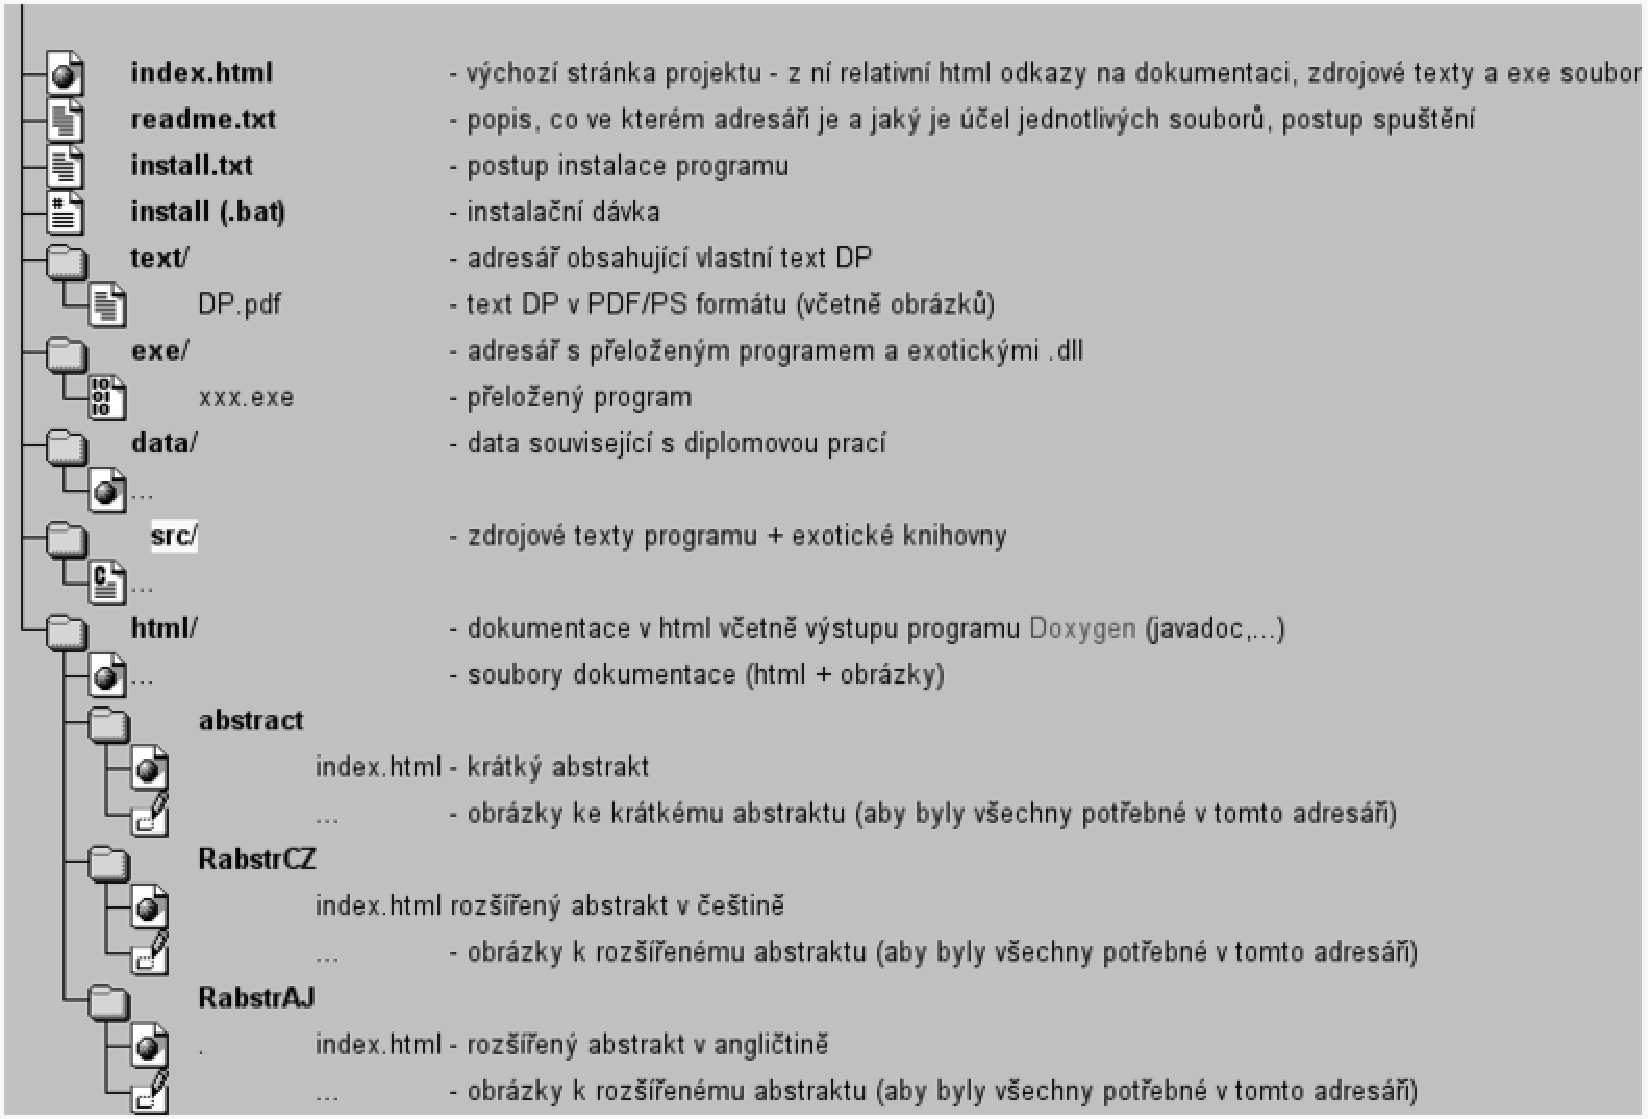
\includegraphics[width=14cm]{figures/seznamcd}
\caption{Seznam přiloženého CD --- příklad}
\label{fig:seznamcd}
\end{center}
\end{figure}

Na GNU/Linuxu si strukturu přiloženého CD můžete snadno vyrobit příkazem:\\ 
\verb|$ tree . >tree.txt|\\
Ve vzniklém souboru pak stačí pouze doplnit komentáře.

Z \textbf{README.TXT} (případne index.html apod.)  musí být rovněž zřejmé, jak programy instalovat, spouštět a jaké požadavky mají tyto programy na hardware.

Adresář \textbf{text}  musí obsahovat soubor s vlastním textem práce v PDF nebo PS formátu, který bude později použit pro prezentaci diplomové práce na WWW.

\end{document}
